\RequirePackage{currfile}
\ifcurrfilename{arxiv-sort.tex}%
{\documentclass[acmsmall,nonacm,natbib=false]{acmart}}
{\documentclass[acmsmall,anonymous,screen,review,natbib=false]{acmart}}
\settopmatter{printfolios=false,printccs=false,printacmref=false}

%% Rights management information.  This information is sent to you
%% when you complete the rights form.  These commands have SAMPLE
%% values in them; it is your responsibility as an author to replace
%% the commands and values with those provided to you when you
%% complete the rights form.
\setcopyright{none}
\copyrightyear{2024}
\acmYear{2024}
% \acmDOI{XXXXXXX.XXXXXXX}

%% These commands are for a PROCEEDINGS abstract or papier.
\acmConference[ICFP'24]{International Conference on Functional Programming}{Sep 2--7, 2024}{Milan, Italy}
%%
%%  Uncomment \acmBooktitle if the title of the proceedings is different
%%  from ``Proceedings of ...''!
%%
%%\acmBooktitle{Woodstock '18: ACM Symposium on Neural Gaze Detection,
%%  June 03--05, 2018, Woodstock, NY}
% \acmPrice{15.00}
% \acmISBN{978-1-4503-XXXX-X/18/06}

%%
%% Submission ID.
%% Use this when submitting an article to a sponsored event. You'll
%% receive a unique submission ID from the organizers
%% of the event, and this ID should be used as the parameter to this command.
%%\acmSubmissionID{123-A56-BU3}

%%
%% For managing citations, it is recommended to use bibliography
%% files in BibTeX format.
%%
%% You can then either use BibTeX with the ACM-Reference-Format style,
%% or BibLaTeX with the acmnumeric or acmauthoryear sytles, that include
%% support for advanced citation of software artefact from the
%% biblatex-software package, also separately available on CTAN.
%%
%% Look at the sample-*-biblatex.tex files for templates showcasing
%% the biblatex styles.
%%
% \bibliographystyle{ACM-Reference-Format}
\RequirePackage[
  % datamodel=acmdatamodel,
  style=acmauthoryear,
  sortcites=true,
  sorting=ynt,
  backend=biber,
  ]{biblatex}

\addbibresource{../symmetries.bib}

%%
%% The majority of ACM publications use numbered citations and
%% references.  The command \citestyle{authoryear} switches to the
%% "author year" style.
%%
%% If you are preparing content for an event
%% sponsored by ACM SIGGRAPH, you must use the "author year" style of
%% citations and references.
%% Uncommenting
%% the next command will enable that style.
% \citestyle{acmauthoryear}

\usepackage{currfile}
\ifcurrfilename{icfp24-sort-strip.tex}%
{\usepackage[appendix=strip,bibliography=common]{apxproof}}%
{\usepackage[appendix=append,bibliography=common]{apxproof}}
\usepackage[useregional]{datetime2}

%% figures
\usepackage{subcaption}
\usepackage{float}
\usepackage{afterpage}
%\usepackage[section,above]{placeins}

%% tikz
\usepackage{tikz}
\usepackage{xifthen}

%% math
\let\Bbbk\relax
\usepackage{amsmath,amsfonts,amsthm,amssymb}
\usepackage{newtxmath}
\usepackage{bbold}
\usepackage{mathpartir}
\usepackage{stmaryrd}
\usepackage{quiver}
\usepackage{ebproof}
\usepackage{listings}

\lstset{%
  basicstyle=\ttfamily,
  columns=fullflexible,
  keepspaces=true,
  mathescape=true,      % Allow escaping to LaTeX math mode within $$
  escapechar=\%,        % Set the escape character (e.g., % for LaTeX commands)
}


%% typesetting
%% fancy quotation
\usepackage[
  style=english,
  english=american,
  french=guillemets,
  autopunct=true,
  csdisplay=true
]{csquotes}
%% customize quote margins
\newenvironment*{innerquote}
  {\setlength{\leftmargini}{0.2cm}%
   \quote}
  {\endquote}
\SetBlockEnvironment{innerquote}

%% special hyphenation
\hyphenation{
  sorting
}
%% tweak hyphenation
\tolerance=9999
\emergencystretch=10pt
\hyphenpenalty=10000
\exhyphenpenalty=100
%% microtypography
\usepackage{microtype}

%% custom macros
\usepackage{hott}
\usepackage{math}
\usepackage{code}
\usepackage{macros}

%%
%% end of the preamble, start of the body of the document source.
\begin{document}

%%
%% The "title" command has an optional parameter,
%% allowing the author to define a "short title" to be used in page headers.
\title{Symmetries in Sorting?}
\subtitle{Last updated on \DTMnow}

%%
%% The "author" command and its associated commands are used to define
%% the authors and their affiliations.
%% Of note is the shared affiliation of the first two authors, and the
%% "authornote" and "authornotemark" commands
%% used to denote shared contribution to the research.
\author{Anonymous}
\orcid{0000-0000-0000-0000}
\affiliation{
  \department{Department of Ordinateur Science}
  \institution{University of Algebra}
  \city{ALgebra City}
  \postcode{10000}
  \country{USA}
}
\email{a@a.edu}

%%
%% By default, the full list of authors will be used in the page
%% headers. Often, this list is too long, and will overlap
%% other information printed in the page headers. This command allows
%% the author to define a more concise list
%% of authors' names for this purpose.
\renewcommand{\shortauthors}{Last updated on \DTMnow}

%%
%% The abstract is a short summary of the work to be presented in the
%% article.
\begin{abstract}
  Sorting algorithms are one of the most common algorithms in functional programming.
Previous works have investigated the correctness of sorting algorithms in terms of
total orders and category theory. 

We provide another perspective on the correctness of sorting algorithms with
universal algebra by understanding it in terms of surjective functions from
free monoids to free commutative monoids, leveraging the power of cubical
type theory to implement theses ideas.
\end{abstract}

%%
%% The code below is generated by the tool at http://dl.acm.org/ccs.cfm.
%% Please copy and paste the code instead of the example below.
%%
\begin{CCSXML}
  <ccs2012>
  <concept>
  <concept_id>10003752.10003790.10011740</concept_id>
  <concept_desc>Theory of computation~Type theory</concept_desc>
  <concept_significance>500</concept_significance>
  </concept>
  <concept>
  <concept_id>10003752.10010124.10010131.10010137</concept_id>
  <concept_desc>Theory of computation~Categorical semantics</concept_desc>
  <concept_significance>500</concept_significance>
  </concept>
  <concept>
  <concept_id>10003752.10010124.10010131.10010133</concept_id>
  <concept_desc>Theory of computation~Denotational semantics</concept_desc>
  <concept_significance>500</concept_significance>
  </concept>
  <concept>
  <concept_id>10011007.10011006.10011008.10011009.10011012</concept_id>
  <concept_desc>Software and its engineering~Functional languages</concept_desc>
  <concept_significafnce>500</concept_significance>
  </concept>
  <concept>
  <concept_id>10011007.10011006.10011039.10011040</concept_id>
  <concept_desc>Software and its engineering~Syntax</concept_desc>
  <concept_significance>500</concept_significance>
  </concept>
  <concept>
  <concept_id>10011007.10011006.10011039.10011311</concept_id>
  <concept_desc>Software and its engineering~Semantics</concept_desc>
  <concept_significance>500</concept_significance>
  </concept>
  </ccs2012>
\end{CCSXML}

\ccsdesc[500]{Theory of computation~Type theory}
\ccsdesc[500]{Theory of computation~Categorical semantics}
\ccsdesc[500]{Theory of computation~Denotational semantics}
\ccsdesc[500]{Software and its engineering~Functional languages}
\ccsdesc[500]{Software and its engineering~Syntax}
\ccsdesc[500]{Software and its engineering~Semantics}

%%
%% Keywords. The author(s) should pick words that accurately describe
%% the work being presented. Separate the keywords with commas.
\keywords{category theory, type theory, semantics}
%% A "teaser" image appears between the author and affiliation
%% information and the body of the document, and typically spans the
%% page.

%%
%% This command processes the author and affiliation and title
%% information and builds the first part of the formatted document.
\maketitle

\begin{acks}
\end{acks}

\section{Introduction}
\label{sec:introduction}

Consider a puzzle about sorting,
inspired by Dijkstra's Dutch National Flag problem~\cite[Ch.14]{dijkstraDisciplineProgramming1997}.
Suppose there are balls of three colors,
corresponding to the colors of the Dutch flag: red, white, and blue.
\[
  \{
  \tikz[anchor=base, baseline]{%
    \foreach \x/\color in {1/red,2/white,3/blue} {
        \node[circle,draw,fill=\color,line width=1pt] at (\x,0) {\phantom{\tiny\x}};
        \ifthenelse{\NOT 1 = \x}{\node at ({\x-0.5},0) {,};}{}
      }
  }
  \}
\]
Given an unordered list of such balls, how many ways can you sort them into the Dutch flag?
\[
  \{
      \tikz[anchor=base, baseline]{%
        \foreach \x/\color in {1/red,2/red,3/blue,4/white,5/blue,6/red,7/white,8/blue} {
            \node[circle,draw,fill=\color,line width=1pt] at (\x,0) {\phantom{\tiny\x}};
            \ifthenelse{\NOT 1 = \x}{\node at ({\x-0.5},0) {,};}{}
          }
      }
    \}
\]
Obviously there is only one way, which is given by the order
$\term{red} < \term{white} < \term{blue}$.
\[
  [
      \tikz[anchor=base, baseline]{%
        \foreach \x/\color in {1/red,2/red,3/red,4/white,5/white,6/blue,7/blue,8/blue} {
            \node[circle,draw,fill=\color,line width=1pt] at (\x,0) {\phantom{\tiny\x}};
            \ifthenelse{\NOT 1 = \x}{\node at ({\x-0.5},0) {,};}{}
          }
      }
    ]
\]
What if we are avid enjoyers of vexillology who also want to consider other flags?
We might ask: how many ways can we sort our unordered list of balls?
We know that there are only $3! = 6$ permutations of
$\{\term{red}, \term{white}, \term{blue}\}$, so there are only 6 possible orderings we can define.
In fact, there are exactly 6 such categories of tricolor flags (\href{https://en.wikipedia.org/wiki/List_of_flags_with_blue,_red,_and_white_stripes#Triband}{Wikipedia}).
We have no allegiance to any of the countries presented by the flags, hypothetical or otherwise -- this is purely combinatorics!
\vspace{0.5em}
\begin{center}
    \foreach \colorA/\colorB/\colorC in {red/white/blue, red/blue/white, white/red/blue, white/blue/red, blue/red/white, blue/white/red}{
    \begin{tikzpicture}[scale=0.5]
    \begin{flagdescription}{3/4}
    \hstripesIII{\colorA}{\colorB}{\colorC}
    \framecode{}
    \end{flagdescription}
    \end{tikzpicture}
    }
\end{center}
\vspace{0.5em}

We posit that because there are exactly 6 orderings, we can only define 6 \emph{correct} sorting
functions.% (up to function extensionality).

In more formal terms: let $A = \{\term{red}, \term{white}, \term{blue}\}$
let $\setord(A)$ be the set of orderings on $A$ and let 
 $\setmtol(A)$  be the set of functions $\term{UnorderedList}(A) \to \List(A)$.
There is a function $\otof : \setord(A) \to \setsort(A)$ that maps orderings to
some subset $\setsort(A) \subset \setmtol(A)$ which we call "sort functions":

\begin{center}
    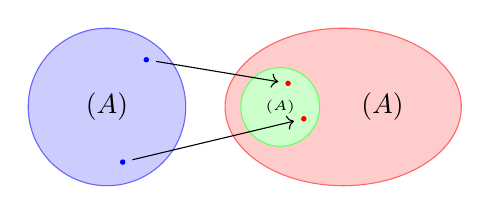
\begin{tikzpicture}
        % draw the sets
        \filldraw[fill=blue!20, draw=blue!60] (-1.5,0) circle (1cm);
        \filldraw[fill=red!20, draw=red!60] (1.5,0) ellipse (1.5cm and 1cm);
        \filldraw[fill=green!20, draw=green!60] (0.7,0) circle (0.5cm);
    
        % the texts
        \node at (-1.5,0) {$\Ord(A)$};
        \node at (0.7, 0) {\tiny$\Sort(A)$};
        \node at (2,0) {$\setmtol(A)$};

    
        % the points in the sets (here I just create nodes to use them later on to position
        % the circles and the arrows
        \node (x1) at (-1,0.6) {};
        \node (x2) at (-1.3,-0.7) {};
        \node (y1) at (0.8,0.3) {};
        \node (y2) at (1,-0.15) {};
    
        % position the elements in the sets (at the nodes we just created)
        \fill[blue] (x1) circle (1pt);
        \fill[blue] (x2) circle (1pt);
        \fill[red] (y1) circle (1pt);
        \fill[red] (y2) circle (1pt);
    
        % draw the arrows
        \draw[->] (x1) -- (y1);
        \draw[->] (x2) -- (y2);
    \end{tikzpicture}
\end{center}

This \textit{seems} trivial to prove: we can construct $\otof(r)$ by parameterizing
any sorting algorithm, e.g.\ insertion sort, by the order relation $r$ and we are done!
This however is not enough: we want to show that there are exactly 6 sorting functions because
there are exactly 6 orderings. In other words, $\setord(A)$ and $\setsort(A)$ should be
isomorphic. There should exist an inverse mapping to $\otof$ that allows us to construct
an ordering $\preccurlyeq$ given a function $s \in \setsort(A)$, such that
$\forall s \in \setsort(A).\, \otof(\otof^{-1}(s)) = s \land \forall r \in \setord(A).\, \otof^{-1}(\otof(r)) = r$.

To complete this proof formally we need to execute the following plan.
\begin{enumerate}
    \item We need to formalize exactly what $\term{UnorderedList}(A)$ and $\List(A)$ are.
    We formalize them in terms of universal algebra: $\term{UnorderedList}(A)$ is 
    the free commutative monoid on $A$ and $\List(A)$ is the free monoid on $A$. We give
    different constructions of them in~\cref{sec:monoids} and ~\cref{sec:commutative-monoids},
    proving these constructions correct by verifying their universal properties.
    We also explore the relationship between commutativity and ordering in
    ~\cref{sec:commutative-monoids} and ~\cref{sec:head},
    showing how imposing commutativity on a free monoid is same as "forgetting" the order,
    giving a formal notion to the idea of unordered list.
    \item We need to nail down exactly what the subset $\Sort(A)$ is. In other words, we need to
    identify what properties functions $f \in \Sort(A) \subset \setmtol(A)$ satisfy which separate
    them from other functions $g \in \setmtol(A)$. We identify two properties in~\cref{sec:sorting},
    giving us two axioms for sorting functions which do not assume a pre-existing total order. This distinguishes our approach 
    from other formalizations of the correctness of sorting such as 
    \cite{appelVerifiedFunctionalAlgorithms2023}.
    \item Using the properties we have identified, we need to construct a full equivalence
    $\Sort(A) \simeq \Ord(A)$. Mapping orders to sorting functions is
    trivial by parameterizing insertion sort on an order relation. More interestingly we need to show how sorting functions
    can be mapped to orders, showing that the properties we have identified for $\Sort(A)$ indeed
    correctly identify the usual notion of sorting functions.
\end{enumerate}

The term "formalize" in the above plan means exactly that, and we therefore need to choose a proof system in which to work. Martin-L\"of Type Theory (MLTT) would not be convenient because of the large amount of work with set quotients and commutativity in our theory. These concepts do not behave well in MLTT and often can only be modelled via setoids. While setoids would suffice for
our purposes, they carry a high proof burden which leads to a
phenomenon (un)affectionately named "setoid hell". We have therefore decided to formalize our proofs
for this paper in Cubical Agda~\cite{vezzosiCubicalAgdaDependently2019}. This allows us to work  naturally with
higher inductive types, and allows for a very simple method of transporting proofs between
different constructions of free algebras by univalence. What also makes Cubical Agda attractive
is that Cubical Type Theory~\cite{cohenCubicalTypeTheory2018}
allows us to enjoy the full power of univalence given by
Homotopy Type Theory~\cite{univalentfoundationsprogramHomotopyTypeTheory2013}, 
without losing canonicity and computational content of the proofs. This means that proofs and functions
transported by univalence actually compute!
We give a table of our formalization in~\cref{sec:formalization}.

% MOVE SOME OF THESE TO DISCUSSION AND OTHER SECTIONS

% Intuitively, what should a correct sorting algorithm do?
% %
% All it knows about balls are their colors, so all it can do is compare balls by color, and move them around.
% %
% A correct sorting algorithm is going to rearrange these balls so the sequence gets partitioned into ``stripes''.
% \[
%   [
%       \tikz[anchor=base, baseline]{%
%         \foreach \x/\color in {1/red,2/red,3/red,4/white,5/white,6/blue,7/blue,8/blue} {
%             \node[circle,draw,fill=\color,line width=1pt] at (\x,0) {\phantom{\tiny\x}};
%             \ifthenelse{\NOT 1 = \x}{\node at ({\x-0.5},0) {,};}{}
%           }
%       }
%     ]
% \]
% There are 3 partitions corresponding to the 3 colors, hence there are $3! = 6$ ways to arrange the partitions.
% %
% Thus, the numbered of correct sorting functions is equal to the number of ways of ordering the colors!
% 
% \redtext{Intuition: what does a correct sorting algorithm do?}
% \begin{itemize}
%     \item It partitions the list by a key, in this case, the colors of the balls.
%     \item The keys need to be totally ordered in order to sort the partitions.
%     \item The number of total orderings will equal the number of possible ways of sorting the sequence.
% \end{itemize}
% \redtext{
%     We will use this simple observation as a motivation, but rather than thinking of it terms of counting, we will go a dimension higher and consider isomorphisms (or bijections) of sets. Is there a connection between the set of total orderings on the carrier set, and the set of correct sorting functions? Our discovery is that there is a bijection between the two! From this observation, we obtain an axiomatic understanding of the correctness of sorting.
% }
% 
% \subsection*{Solving the puzzle}
% 
% Suppose $A$ is the 3-element set $\{a,b,c\}$. There are many possible orderings of these elements,
% eg, $[a,b,c]$, or $[a,c,b]$, $[b,c,a]$, 6 of them.
% Consider lists of $A$, such as $[a,b,c,a,c,b,c,c]$, and we want to sort this list, so we want to write a sort function $s\colon List(A) \to List(A)$.
% Obviously, there would be infinitely many functions $\List(A) \to \List(A)$, but how many of them
% would actually be correct sorting functions? We posit that there are only 6 correct sorting
% functions, and our justification is because there are only 6 possible ordering on $A$.
% But how do we prove this?
% 
% Let's try to write some functions $\List(A) \to \List(A)$, for example:
% \begin{lstlisting}[language=haskell]
% s1 : List A $\to$ List A
% s1 [] = []
% s1 (x :: xs) = if x = a then ... else ...
% \end{lstlisting}
% $s1$ is a sort function only if $A$ is ordered by $a < c < b$.
% In fact, this goes both ways!
% If we write a correct sort function $s$, we will get a total order on $A$.
% We gain our main insight: fixing a permutation on $\{a,b,c\}$ fixes an ordering on the elements which determines a correct sort function for lists of $A$.
% 
% %% Now, suppose you have lists of elements of $A$, such as, $[(a,"foo"), (b, "bar"), (c, "baz")]$, and we want to sort this list using the first element of the tuple as the key -- in how many ways can we sort correctly?
% 
% %% Sorting algorithm is a common algorithm we introduce to undergraduate students
% %% when we teach them algorithmics. For example, a sort algorithm can be a function
% %% $\text{List} \, \mathbb{N} \to \text{List} \, \mathbb{N}$, which produces $[1,2,3,4]$
% %% given the input $[2,3,1,4]$.
% However, how do we formalize the correctness of this sort function?
% The common formalization of a correct sort algorithm is to say a sort algorithm produces
% an "orederd list", for example, one such formalization would be the definition
% from Verified Functional Algorithms \cite{appelVerifiedFunctionalAlgorithms2023}, translated into Agda.
% 
% \begin{lstlisting}[language=Haskell]
% data Sorted : List A $\to$ Type where
%   sorted-nil : Sorted []
%   sorted-one : $\forall$ x $\to$ Sorted [ x ]
%   sorted-cons : $\forall$ x y zs $\to$ x $\leq$ y $\to$ Sorted (y :: zs) $\to$ Sorted (x :: y :: zs)
% \end{lstlisting}
% 
% This is a perfectly valid formalization of an ordered list! Empty lists and singleton lists
% are ordered, and we can inductively construct an "orderness witness" by prepending a new element
% to an ordered list, provided that the new element is less than the head of the old ordered list of
% course. 
% 
% A correct sort function then has the type: \inline{sort : List A -> Sg(xs:List A).Sorted xs}.\vc{How is ours better?}
% This definition, however, assumes an existing total order on $A$. This is
% unsatisfactory, in a way, because a sorting algorithm is fundamentally just a function. Can we
% axiomatize the correctness of a sorting algorithm purely by the properties of functions?
% 
% % \begin{itemize}
% %     \item What exactly is special about commutativity? We study this from the ordinateur science point of view, using monoids and commutative monoids, which are important data structures.
% %     \item In some sense, commutativity or unordering is formally understood as non-determinism, such as in concurrency using finite powersets or free commutative monoids. When can a commutative structure be linearised?
% %     \item Commutativity is a way of enforcing unordering, or forgetting ordering, there are many ways of doing it: by using adjacent transpositions to generate all symmetries, or quotienting by symmetries
% %     \item if you forget the ordering and get an unordered list (or data structure), can you recover the ordering? Of course, it's a sorting algorithm, that is very basic to ordinateur science. In fact, this gives us a specification for sorting, which is our application.
% %     \item Why do we want to write intrinsically verified sorting algorithms?
% %         \begin{itemize}
% %         \item Using HITs, the sort function is correct by construction. This is unlike verifying
% %             sort externally in Coq.
% %         \item Can we structure the program in a better way? This is already solved by the bialgebraic sorting point of view, are we doing anything new?
% %         \item We give a more conceptual understanding of the correctness of sorting algorithms, using an abstract framework.
% %         \item Conventional way: a sort function turns a list into an ordered list.
% %         \item Our way: a sort function is a function satisfying some abstract properties, independent of a given ordering.
% %         \end{itemize}
% % \end{itemize}
% 
% % overall plan: with the universal algebra

% We can now study sorting from an algebraic perspective, viewing sorting as mappings from free commutative
% monoids to free monoids. There are many ways to construct free commutative monoids, such as using adjacent transpositions to generate all symmetries, or quotienting free monoids by symmetries, which we would
% elaborate on in ~\cref{sec:commutative-monoids}, all of which can be very naturally represented
% using higher inductive types in univalent type theory. We also
% create a framework for universal algebra, allowing us to formalize the notion of free algebras and
% their universal property, and finally within the framework we can formalize the axioms of sorting
% algorithms and their relationship to total orders.
% % Univalent type theory and Cubical Agda gives us a
% % rigorous framework for implementing these ideas, and higher inductive types allow us to express
% % the constructions of free commutative monoids very naturally.



\subsubsection*{Outline and Contributions}

\begin{myitemize}
  \item In~\cref{sec:notation}, we describe the notation we use in the paper.
  \item In~\cref{sec:universal-algebra}, we give some background on a categorical framework for universal algebra including equations, and its formalization in HoTT. We give the definition of free algebras and their universal property.
  \item In~\cref{sec:monoids}, we give various constructions of free monoids, and their proofs of universal property.
  \item In~\cref{sec:commutative-monoids}, we add commutativity to free monoids, and show how to extend the proofs of universal property appropriately. Using our results we prove existing constructions
  of free commutative monoid are correct directly by their universal property, as opposed to
  the more common method of proving their correctness by isomorphism to known constructions
  of free commutative monoid.
  \item In~\cref{sec:combinatorics}, we show how free monoids and free commutative monoids are different, by discussing various combinatorial properties and operations, which can be defined for both, and ones which cannot be defined for both.
  \item In \cref{sec:sorting}, we build on the constructions of the previous sections and study intrinsically verified sorting function. The main result in this section is to connect total orders and sorting and commutativity, by proving an equivalence between decidable total orders on a carrier set $A$, and correct sorting algorithms on lists of elements of $A$.
  \item All the work in this paper is formalized in Cubical Agda, which is discussed in~\cref{sec:formalization}, and the accompanying code is available as supplementary material. Although the formalization is a contribution in itself, the purpose of the paper is not to discuss the formalization, but to present the results in un-formalized form, using HoTT/UF as a foundation, so the ideas are accessible to a wider audience, even without a background in type theory or formalization.
  \item In~\cref{sec:discussion}, we discuss connections to related work, and future work.
\end{myitemize}
 %% 2.5 pages
\section{Type Theory}\label{sec:type-theory}
As we have explained, our work is formalized in Cubical Agda and Cubical Type Theory,
which is a variant of Homotopy Type Theory that is designed to preserve
computational properties of type theory.
We refer the readers to other works such as~\cite{vezzosiCubicalAgdaDependently2019}
and~\cite{cohenCubicalTypeTheory2018} for a more in-depth explanation on Cubical Type Theory
and how we can program in Cubical Agda.
We also give an overview of relevant features
in Cubical Type Theory which normal type theory (namely MLTT) lacks, and how these features
are used within the scope of our work.
\subsection{Dependent Types}
We first review some basic ideas from type theory. We assume the readers
have experience with dependent typed programming, so this would only
serves as a refresher.
\subsubsection{$\Pi$-types}
$\Pi$-types generalizes function types.
These types capture the idea of functions that can take different types
as input or return different types as output depending on the input.
The type of a function that accepts an argument $x: A$ and returns
an element of type $B(x)$, where $B$ might depend on $x$,
can be expressed as $(x: A) \to B(x)$ or $\Pi_{(x: A)} B(x)$.

\subsubsection{$\Sigma$-types}
$\Sigma$-types generalizes product types. 
These types represent tuples where the type of the second component
depends on the first. An element of the type
$\Sigma_{(x: A)} B(x)$ is a pair $(a, b)$
where $a$ is of type $A$ and $b$ is of type $B(a)$.

\subsubsection{Identity types}
The identity type of a type $A$ expresses equality in type theory.
If $a$ and $b$ are elements of type $A$, then the type expressing that
$a$ is equal to $b$ is often written $a =_A b$. Optionally, the type can
be omitted for brevity, therefore written just as $a = b$. This is
often useful to state when two elements should be equal but they are not
definitionally equal. For example, given $n : \Nat$, the elements
$n + 0 : \Nat$ and $0 + n : \Nat$ should be the same, however depending
on the implementation of $+$ they may not be definitionally equal,
therefore $B(n + 0)$ and $B(0 + n)$ would give us different types
definitionally. Having a type $n + 0 =_\Nat 0 + n$ would allow us to
convert $x : B(n + 0)$ to $x : B(0 + n)$ and vice versa, therefore
solving the over-restriction of definitional equality.

\subsubsection{Propositions as Types}
The Curry-Howard correspondence gives us the propositions-as-types
principle, which states that propositional logic can be interpreted
as types:
\begin{itemize}
    \item A type $P$ can be viewed as a proposition, and a term of that
    type is a proof of the proposition.
    \item $\Pi$-types correspond to universal quantification or implications.
    A function $f : P \to Q$ can be thought of as "$P$ implies $Q$", and
    a function $f : (a : A) \to P(a)$ can be thought of as "for all $a$
    of type $A$, $P(a)$ holds".
    \item $\Sigma$-types correspond to existential quantification.
    An element of $\Sigma_(a : A)\,P(a)$ can be thought of as a proof
    that states "there exists an $a$ of type $A$ such that $P(a)$ holds".
\end{itemize}

\subsection{Homotopy Types}
In Homotopy Type Theory, types are assigned a homotopy level
(often abbreviated h-level). I will explain the concept of h-level
since it is important to understand the terminlogy used in the rest
of the dissertation.
\subsubsection{Contractible Type}
A type $A$ is said to be contractible iff there is an element
$a : A$, refered to as the \emph{center of contraction}, such that
for all $x: A$, we have $a = x$. More formally:
\begin{align*}
    \term{isContr}(A) := \Sigma_{(a : A)}\Pi_{(x : A)}(a =_A x).
\end{align*}
Contractible types are assigned the h-level 0.
One example of such a type would be the unit type $\unitt$.
In fact, all contractible types are equivalent to $\unitt$.
\subsubsection{Mere proposition}
Going one dimension higher, we have mere propositions. A type $A$
is said to be a mere proposition iff all elements of $A$ are equal.
We give two formal and equivalent definitions:
\begin{align*}
    \term{isProp}(A) & := \Pi_{(x,y : A)}(x =_A y).\\
    \term{isProp}(A) & := \Pi_{(x,y : A)}\term{isContr}(x =_A y).
\end{align*}
Mere propositions are assigned the h-level 1.
We use $\hProp := \Sigma_\UU \term{isProp}.$ to denote the type for
all types that are propositions.
Examples of such types
are the unit type $\unitt$ and the empty type $\emptyt$. In HoTT,
we use the adverb \emph{merely} to describe propositions represented
as a mere propositional type. We also introduce the idea of
propositional truncation, where a type $A$ is truncated to 
a mere propositional type $\norm{A}$. This can be done with a higher
inductive type (elaborated more in~\cref{sec:HIT}):

\begin{code}
data [[_]] (A : UU) : UU where
    [_]  : A -> [[A]]
    trunc : (x, y : [[A]]) -> x = y
\end{code}
One example usage of propositional truncation is the definition of
\emph{mere existence}, where $\exists (x: A).\,P(x)$ is represented
as $\norm{\Sigma_{(x:A)}P(x)}$. This differs from $\Sigma_{(x:A)}P(x)$
in that mere existence only contains information whether such an $x$
that satifies $P$ exists, whereas the $\Sigma$ type contains more information,
namely the value of the actual element $x$. This makes it such that
with a mere existential proof of $x$ we would only be able to use $x$
to prove other mere propositions, but we would not be able to define
any functions that actually depend on the value of $x$. For example,
consider a function $f : (x : A) \to P(x) \to \Nat$ which takes an $x: A$
that satisfies $P$ and return a $\Nat$. Given $\exists x.\,P(x)$ we would
not be able to apply $f$ on $x$, since $\Nat$ is not a proposition. 
On the other hand, assuming we have another mere proposition
$Q : A \to \hProp$, and a proof that $\forall y.\,P(y) \to Q(y)$, 
we can use $\exists x.\,P(x)$ to prove $\exists x.\,Q(x)$.

\subsubsection{Sets}
Going one dimension higher, we have sets. A type $A$ is said to be a set
iff the identity type of $A$ is a mere proposition.
\begin{align*}
    \term{isSet}(A) := \Pi_{(x,y : A)}\term{isProp}(x =_A y).
\end{align*}
Sets are assigned the h-level 2.
We use $\hSet := \Sigma_\UU \term{isSet}.$ to denote the type for
all types that are sets.
Examples of sets would be $\Nat$, the boolean type $\boolt$, and also
the unit and empty type $\unitt$ and $\emptyt$. The type for all types
that are mere propositions $\hProp$ is also a set.

We note that in type theories with K-axiom or uniqueness of identity proofs
(UIP), all types are sets. For example, in Idris2~\cite{brady_idris_2021},
we can prove this
by pattern matching on proofs:
\begin{code}
uip : (A : Type) -> (x, y : A) -> (p, q : x = y) -> p = q
uip A x x Refl Refl = Refl
\end{code}

The K elimination rule allows us to pattern match on identity types and force
them to be $\term{Refl}$, thus allowing us to prove $p = q$ since both
$p$ and $q$ are $\term{Refl}$. HoTT, however, does not assume the K-axiom,
therefore this would be invalid in HoTT.

In the dissertation we would be primarily working with sets
(and mere propositions since all mere propositions are sets).
There are higher dimensional types, but generalizing the work to
higher dimensions is currently left for future works.

\subsubsection{Groupoid}
Going one dimension higher, we have groupoids. A type $A$ is said to be a
groupoid iff the identity type of $A$ is a set.
\begin{align*}
    \term{isGroupoid}(A) := \Pi_{(x,y : A)}\term{isSet}(x =_A y).
\end{align*}
Groupoids are assigned the h-level 3. All sets are groupoids,
and the type for all types that are sets $\hSet$ is also a groupoid.
For example, consider the boolean type $\boolt : \hSet$. There are two
different elements of $\boolt =_\hSet \boolt$, which generated by
univalence (elaborated more in~\cref{types:univalence}) from two
different equivalence we can define on $\boolt$ to $\boolt$, the
identity function $id$ and the negate functon $not$.
This shows that $\boolt =_\hSet \boolt$ is \emph{not} a mere proposition,
therefore $\hSet$ is \emph{not} a set. This shows how K-axiom is
incompatible with univalence and HoTT.

\subsubsection{n-Types}
We can define further higher dimensional types by induction, giving us
2-groupoids, 3-groupoids, and so on. More generally, we can define
n-types as below, with $n$ starting at -2.
\begin{align*}
    \term{is-n-type}(A) := \begin{cases}
        \term{isContr}(A) & \text{if $n = -2$} \\
        \prod_{x, y : A}\term{is-(n-1)-type}(x =_A y) & \text{otherwise}
    \end{cases}
\end{align*}

Somewhat confusingly, (-2)-types (contractible types) have h-level 0,
and (-1)-types (mere propositions) have h-level 1, and so on.
In the lingo of HoTT, when we say n-types we start counting from -2,
but for h-levels we start counting from 0. This is because when
the concept of h-level is invented Voevodsky chose to start counting
from 0~\cite{voevodsky_univalent_2010},
but the idea of n-trunction originates earlier from $\inf$-category theory,
where truncation level starts from -2~\cite{lurie_higher_2008}.

\subsection{Function Extensionality}
Function extensionality $\term{funExt}$ states that given two functions $f$ and $g$,
$\term{funExt}: \forall x.\,f(x) = g(x) \to f = g$. MLTT by itself does not have $\term{funExt}$,
instead it has to be postulated as an axiom, thereby losing canonicity, in other words,
we would not be able to compute any constructions of elements that involve $\term{funExt}$
in its construction. In Cubical Type Theory, we can derive $\term{funExt}$
as a theorem while also preserving canoncity, therefore we can compute with constructions
involving $\term{funExt}$!

Within the scope of our work, $\term{funExt}$ is heavily used in
~\cref{mon:array} and~\cref{cmon:bag}, where a $n$-element array $A^n$ is defined as lookup functions
$\Fin[n] \to A$. Therefore, to prove two arrays are equal, we need to show that two functions would be
equal, which is impossible to do without $\term{funExt}$. We also would not be able to normalize
any constructions of arrays which involve $\term{funExt}$ if it is postulated as an axiom, therefore
the computational property of Cubical Type Theory is really useful for us.

\subsection{Higher Inductive Types}\label{sec:HIT}
Higher inductive types
allow us to extend inductive types to not only allow point constructors
but also path constructors, essentially equalities between elements of the HIT. One such example
would be the following definition of $\mathbb{Z}$:

\vspace{-1em}
\begin{code}
data $\mathbb{Z}$ : UU where
    pos : (n : $\mathbb{N}$) -> $\mathbb{Z}$
    neg: (n : $\mathbb{N}$) -> $\mathbb{Z}$
    posneg : pos 0 == neg 0
\end{code}
\vspace{1em}

The integers are often represented with a $\term{pos} : \Nat \to \mathbb{Z}$
and $\term{negsuc} : \Nat \to \mathbb{Z}$, where natural numbers
are mapped into the integers via the $\term{pos}$ constructor, and negative numbers are constructed
by mapping $n : \Nat$ to $-(n + 1)$. The shifting by one is done to avoid having duplicate elements
for 0, which can easily lead to confusion. HIT allows us to define integers more naturally by saying
$\term{pos}(0) = \term{neg}(0)$, avoiding the confusing shift-by-one hack.

With HITs we can define a general data type for set quotients:
\begin{code}
data _/_ (A : UU) (R : A -> A -> UU) : UU where
    [_]  : A -> A / R
    q/ : (a b : A) -> (r : R a b) -> [ a ] == [ b ]
    trunc : (x y : A / R) -> (p q : x = y) -> p = q
\end{code}

The $\term{q/}$ constructor says if $a$ and $b$ can be identified by a relation $R$, then
they should belong to the same quotient generated by $R$.
One might also notice the $\term{trunc}$ constructor, which says and proofs of $x =_{A/R} y$ are equal.
This constructor basically truncates the $\term{\_/\_}$ type down to set, so that we do not have to
concern ourselves with higher paths generated by the $\term{q/}$ constructor.
We give a more precise definition of "set" in Homotopy Type Theory and examples of types that are
higher dimension than sets in~\cref{types:univalence}.

In our work, higher inductive types and set quotients are used extensively to define commutative
data structures, which we would demonstrate in~\cref{sec:commutative-monoids}. In MLTT we can only
reason with quotients and commutativity by setoids, which comes with a lot of proof burden
since we cannot work with the type theory's definition of equalities and functions directly,
instead we have to define our own equality relation and define our own type for setoid homomorphisms,
giving rise to the infamous setoid hell.

\subsection{Univalence}\label{types:univalence}
In MLTT we cannot construct equalities between types. Univalence, the core of Homotopy Type Theory,
gives us equalities between types by the univalence axiom. To see how this is useful,
consider $A, B : \mathcal{U}, P : \mathcal{U} \rightarrow \mathcal{U}, A = B$, we can
get $P(B)$ from $P(A)$ by transport (or substitution).  

To define univalence, we first need to define the notion of equivalence:
\begin{definition}[Equivalence]
    A function $f : A \to B$ is said to be an equivalence
    function iff it has a left inverse $g : B \to A$ and right inverse 
    $h : B \to A$ such that
    $(\forall x.\, g(f(x)) = x) \land (\forall x.\, f(h(x)) = x)$. 
    Two types $A$ and $B$ are said to be equivalent iff there exists
    an equivalence function $f : A \to B$. 
\end{definition}

We note that the definition of equivalence is very similar to
an isomorphism, only differing in that an equivalence can have
different functions for left and right inverse, whereas an isomorphism
would have the same function, therefore making it just an (ordinary) inverse.

Assuming $A$ (and subsequently $B$ by equivalence) is a $\hSet$,
$f$ being a equivalence function would imply it is an isomorphism and 
vice versa, thus making both definitions the same. However, for higher
dimensional types, these two definitions would not necessarily imply
each other.
More explicitly: let $\term{qinv}(f)$
be the witness on $f$
stating $f$ is an isomorphism, and $\term{isequiv}(f)$ be the witness on
$f$ stating $f$ is an equivalence function.
\begin{align*}
\term{qinv}(f) & = \Sigma_{g : B \to A}(f \comp g \sim id)\times(g \comp f \sim id) \\
\term{isequiv}(f) & = (\Sigma_{g : B \to A}(f \comp g \sim id))\times(\Sigma_{h : B \to A}(h \comp f \sim id))
\end{align*}
$\term{isequiv}(f)$ is a mere proposition while $\term{qinv}(f)$ is not
necessarily a mere proposition.
We refer the readers
to~\cite[Chapter 4.1]{univalentfoundationsprogramHomotopyTypeTheory2013} for a proof.

\begin{definition}[Univalence axiom]
    $(A = B) \simeq (A \simeq B)$
\end{definition}
Essentially, if we can construct an equivalence between two types $A$ and $B$,
we can obtain a equality of the types $A$ and $B$. While in HoTT we cannot
compute with elements constructed with univalence since it is postulated as an
axiom, Cubical Type Theory allows us to derive univalence as a computable
theorem, therefore we can transport functions and proofs from one type to
another freely without worrying about terms not being able to normalize!

Within the scope of our work, since we have multiple constructions of free monoids
and free commutative monoids, given in~\cref{sec:monoids} and~\cref{sec:commutative-monoids},
having univalence allows us to easily transport proofs and functions from one construction to another.
Another instance where univalence is used is the definition of membership proofs in~\cref{comb:member},
where we want to show to propositions are commutative: i.e. $\forall p, q: \hProp, p \vee q = q \vee p$.
Since $p$ and $q$ are types, we need univalence to show $p \vee q = q \vee p$ are in fact equal.

\section{Notation}\label{sec:notation}
We give a quick overview of the notations used in this paper.

We denote the type of types with $\mathcal{U}$. 
In practice, $\mathcal{U}$ would be indexed by a type level 
à la Russell for consistency, however we opted to omit the type level
for simplicity and clarity.
We use $\Fin[n]$ to denote finite sets of cardinality $n$ in HoTT~\cite{yorgeyCombinatorialSpeciesLabelled2014a}.
This is defined as follows:

\begin{code}
Fin : $\mathbb{N}$ -> UU
Fin n = $\Sigma$[ m $\in$ $\mathbb{N}$ ] (m < n)
\end{code}

There are other ways to define $\Fin$, most notably as an indexed inductive type:
\begin{code}
data Fin : $\mathbb{N}$ -> UU where
    fzero : {k : $\mathbb{N}$} -> Fin (suc k)
    fsuc : {k : $\mathbb{N}$} -> Fin k -> Fin (suc k)
\end{code}


In our construction we opted to use the $\Sigma$-type definition
because cubical Agda does not behave well
when pattern matching on indexed inductive types.

We also use $\times$ to denote product types and $+$ to denote coproduct types.
For mere propositions, we use $\land$ to denote logical and, and $\vee$ to denote logical or.
In Cubical Agda these are defined as propositionally-truncated products and coproducts.
We also use $\exists$ to denote mere existence, which is defined as
propositionally-truncated $\Sigma$-types are shown above. %% 1 page
\label{sec:universal-algebra}

As explained above, we can formalize the notion of an unordered list
as the free commutative monoid and the idea of a list as the free
monoid. We can then study sorting as a relationship between these
two structures under the framework of universal algebra~\cite{birkhoffStructureAbstractAlgebras1935}.
However, to begin, we would need to explain what an algebra is,
what exactly is the definition of "free".

\section{Algebra}\label{algebra:signature}
First we define very generally what an algebra is. Every algebra
has a signature $\sigma$, which is a (dependent) tuple of:
\begin{itemize}
    \item a set of function symbols $op : \Set$,
    \item and an arity function $ar : op \to \Set$.
\end{itemize}

Here, $op$ gives us a set of names to refer to the operations we can do
in an algebra, and the arity function $ar$ specifies the arity of the operation,
using the cardinality of the output set as the arity. In other definitions,
the arity function may be defined as $ar : op \to \Nat$, which specifies
the arity of an operation $op$ by the output natural number. However,
for generality, we decide to use $\hSet$ and cardinality for arity instead,
so that we can have operations of infinite arity. 

\begin{example}
We can define the signature of monoid as follow: the algebra $\Mon$
has operation symbols $\{ e, \mult \}$, referring to the identity operation
and the multiplication operation. The arity function is defined as:
$ar := \{ e \mapsto \Fin[0], \mult \mapsto \Fin[2] \}$.
\end{example}

We use $X^Y$ to denote a vector of $X$ from now on, with the dimension of
the vector given by the cardinality of $Y$. We now can define the type
$F_\sigma(X) := \Sigma_{(f: op)}X^{ar(f)}$, which would be an endofunctor
on $\Set$. We refer to this endofunctor as the signature endofunctor.
In plain English, $F_\sigma(X)$ is a tuple of an operation symbol $op$
and a vector of $X$, where the dimension of the vector is the arity of $op$.

\begin{definition}\label{algebra:struct}
    A $\sigma$-structure $\mathfrak{X}$ is an $F_\sigma$-algebra, given by a tuple
    of:
    \begin{itemize}
        \item a carrier set $X : \hSet$,
        \item and an interpretation function $\alpha_X : F_\sigma(X) \to X$.
    \end{itemize}
\end{definition}

In the rest of the dissertation, we use a normal alphabet
(e.g. $X$) to denote the carrier set, and the alphabet in Fraktur font
(e.g. $\mathfrak{X}$) to denote an algebra based on the carrier set.

\begin{example}
($\Nat$, +) is a $\term{Mon}$-algebra, with
the carrier set given by $\Nat$ and its interpretation function given by:
\begin{align*}
    \alpha_X(e) & = 0 \\
    \alpha_X(\mult, [a, b]) & = a + b
\end{align*}
\end{example}

\begin{definition}
    A $F_\sigma$-algebra homomorphism $h: X \rightarrow Y$ is a function such that:
% https://q.uiver.app/#q=WzAsNCxbMCwwLCJGX3tcXHNpZ21hfShYKSJdLFsxLDAsIlgiXSxbMCwxLCJGX3tcXHNpZ21hfShZKSJdLFsxLDEsIlkiXSxbMCwxLCJcXGFscGhhX1giXSxbMCwyLCJGX3tcXHNpZ21hfShoKSIsMl0sWzIsMywiXFxhbHBoYV9ZIiwyXSxbMSwzLCJoIl1d
\[\begin{tikzcd}[ampersand replacement=\&,cramped]
	{F_{\sigma}(X)} \& X \\
	{F_{\sigma}(Y)} \& Y
	\arrow["{\alpha_X}", from=1-1, to=1-2]
	\arrow["{F_{\sigma}(h)}"', from=1-1, to=2-1]
	\arrow["{\alpha_Y}"', from=2-1, to=2-2]
	\arrow["h", from=1-2, to=2-2]
\end{tikzcd}\]
\end{definition}

Informally, this means that for any $n$-ary function symbol $(f, [x_1, \dots, x_n]) : F_{\sigma}(X)$,
\begin{align*}
    h(\alpha_X(f, [a_1, \dots, a_n])) = \alpha_Y(f, [h(x_1), \dots, h(x_n)])
\end{align*}

$F_{\sigma}$-algebras and their morphisms form a category $F_\sigma$-Alg.
For brevity, we also refer to this category as $\sigma$-Alg. The category
is given by the identity homomorphism and composition of homomorphisms.

\section{Free Algebra}\label{sec:universal-algebra:free-algebras}
The category $\sigma$-Alg admits a forgetful functor
$\sigma-\term{Alg} \to \Set$, which forgets all the algebraic structure
and only retains the underlying carrier set.
We use $U$ to denote the forgetful functor, and under our notation
$U(\mathfrak{X})$ is simply $X$.

The free $\sigma$-algebra $\mathfrak{F}$ is simply defined as the left adjoint to $U$.
More concretely, it is given by:
\begin{itemize}
    \item a type constructor $F : \Set \to \Set$,
    \item a universal generators map $\eta_X : X \to F(X)$, such that
    \item for any $\sigma$-algebra $\mathfrak{Y}$, post-composition with $\eta_X$ is an equivalence:
\end{itemize}
\[
\begin{tikzcd}[ampersand replacement=\&]
	\mathfrak{F}(X) \\
	\\
	\mathfrak{Y}
	\arrow["f", dotted, from=1-1, to=3-1]
\end{tikzcd}
\mapsto
\begin{tikzcd}[ampersand replacement=\&]
	X \&\& {F(X)} \\
	\\
	\&\& {Y}
	\arrow["\eta_X", color={rgb,255:red,255;green,54;blue,51}, from=1-1, to=1-3]
	\arrow["f \comp \eta_X"', from=1-1, to=3-3]
	\arrow["{f}", dotted, from=1-3, to=3-3]
\end{tikzcd}\]

More concretely, let $f$ be a morphism from $\mathfrak{F}(X) \to \mathfrak{Y}$.
$f$ would be a homomorphism since $\mathfrak{F}(X)$ and $\mathfrak{Y}$ are
objects in the category $\sigma$-Alg. 
We use
$\blank \comp \eta_X : (\mathfrak{F}(X) \to \mathfrak{Y}) \to (X \to Y)$
to denote the act of turning a homomorphism to a set function by
post-composition with $\eta_X$.
The universal property of free algebras state that $\blank \comp \eta_X$
is a equivalence, i.e. there is a one-to-one mapping from
homomorphisms $\mathfrak{F}(X) \to \mathfrak{Y}$ to set functions $X \to Y$.
Naturally, there would be an inverse mapping which maps set functions $X \to Y$
to homomorphisms $\mathfrak{F}(X) \to \mathfrak{Y}$. We refer to this
as the extension operation $\ext{(\blank)} : (X \to Y) \to (\mathfrak{F}(X) \to \mathfrak{Y})$,
and we use $\ext{f}$ to denote a homomorphism given by a set function $f : X \to Y$.

By definition, if $F : \Set \to \Set$ satisfies the universal property of
free $\sigma$-algebra, then $\mathfrak{F}$ would be the free $\sigma$-algebra.
We use "the" to refer to $F$ since $F$ is unique up to isomorphism. 

\begin{lemma}\label{lem:free-algebras-unique}
Any two free $\sigma$-algebra on the same set are isomorphic.
\end{lemma}
\begin{proof}
Let $E(X)$ and $F(X)$ be the carrier sets of two free $\sigma$-algebras.
This gives us $\eta_1 : X \to E(X)$ and $\eta_2 : X \to F(X)$.
We can extend them to $\ext{\eta_1} : \mathfrak{F}(X) \to \mathfrak{E}(X)$
and  $\ext{\eta_2} : \mathfrak{E}(X) \to \mathfrak{F}(X)$. By uniqueness,
$\ext{\eta_1}$ and $\ext{\eta_2}$ must be the identity homomorphism,
therefore $E(X)$ and $F(X)$ are isomorphic.
\end{proof}

\subsection{Construction}
We can construct the carrier set of the free $\sigma$-algebra
$\mathfrak{F}(X)$ as an inductive type of trees $Tr_\sigma(V)$:
\begin{code}
data Tree (V : UU) : UU where
    leaf : V -> Tree V
    node : F$_\sigma$(Tree V) -> Tree V
\end{code}

The constructors $leaf$ and $node$ correspond to the generator map
and the interpretation function. Concretely, $Tr_\sigma(V)$ can
be thought of as an abstract syntax tree denoting operations done
an elements of $V$. 

Given a $\sigma$-algebra $\mathfrak{X}$, composing a homomorphism
$f : \mathfrak{F}(V) \to \mathfrak{X}$ with $node$ with turn it
into a function $V \to X$.
We can define an inverse to this operation by lifting a set function
$f : V \to X$ to a homomorphism $\ext{f} : \mathfrak{F}(V) \to \mathfrak{X}$
as follow: we first apply $f$ on every leaves of the tree, giving us
$Tr_\sigma(X)$, and evaluate the tree according to the operations
in the nodes, giving us a $X$ as the result.

\begin{example}
A tree for $\sigMon$ with the carrier set $\Nat$ would look like:
\begin{center}
\scalebox{0.7}{
% https://q.uiver.app/#q=WzAsNixbMiwyLCIrIl0sWzIsMywiNCJdLFszLDEsIisiXSxbMiwwLCIxIl0sWzQsMCwiMSJdLFswLDAsIjIiXSxbMCwxXSxbMiwwXSxbMywyXSxbNCwyXSxbNSwwXV0=
\begin{tikzcd}[ampersand replacement=\&,cramped]
	2 \&\& 1 \&\& 1 \\
	\&\&\& {+} \\
	\&\& {+} \\
	\&\&
	\arrow[no head, from=3-3, to=4-3]
	\arrow[from=2-4, to=3-3]
	\arrow[from=1-3, to=2-4]
	\arrow[from=1-5, to=2-4]
	\arrow[from=1-1, to=3-3]
\end{tikzcd}
}
\hspace{2em}
% https://q.uiver.app/#q=WzAsMixbMCwwLCJlIl0sWzAsMiwiMCJdLFswLDFdXQ==
\begin{tikzcd}[ampersand replacement=\&,cramped]
	e \\
	\\
	\arrow[no head, from=1-1, to=3-1]
\end{tikzcd}
\end{center}
    % Some example trees for $\sigMon$, with leaves drawn from $\{\rwb\}$.
    % %
    % \todo{Expand the signature functor and show how this produces binary trees.}
\end{example}

\section{Equation}\label{sec:universal-algebra:equations}
We have shown how to define the operations of an algebra, but we have not
shown how to define the equations of an algebra. For example, a monoid
should satisfy the unit laws and associative law. We now explain how
we can define equations.

Much like operation signatures, every algebra also has an equation signature
$\epsilon$, which is a (dependent) tuple of:
\begin{itemize}
    \item a set of equation symbols $eq : \Set$,
    \item and an arity of free variables $fv : eq \to \Set$.
\end{itemize}

Here, $eq$ gives us a set of names to refer to an equation which
the algebra must satisfy, and the arity function $fv$ specifies the 
number of free variables in the equation, using the cardinality of the
output set as the arity. Once again, other definitions might opt to
define this as $fv : eq \to \Nat$, but we opted to use $\hSet$ and
cardinality instead to allow for infinitary equations.

\begin{example}
We can define the equation signature of monoid as follow: the algebra
$\Mon$ has equation symbols $\{\term{unitl}, \term{unitr}, \term{assocr}\}$,
referring to the unit left law, the unit right law, and the associativity law.
The arity function is defined as:
$fv : \{ \term{unitl} \mapsto \Fin[1], \term{unitr} \mapsto \Fin[1], \term{assocr} \mapsto \Fin[3] \}$.
\end{example}

We can the define a system of equations (or equational theory $T_\epsilon$)
by a pair of trees on the set of free variables, representing the
left hand side and right hand side of the equations.
\begin{definition}
A system of equations $T_\epsilon$ is defined as
$l, r : (e : eq) \to Tr_\sigma(fv(e))$.
\end{definition}

We say a $\sigma$-structure $\mathfrak{X}$ satisfies $T$
iff for all $e : eq$ and
$\rho : fv(e) \to X$, $\ext{\rho}(l(e)) = \ext{\rho}(r(e))$.
Concretely, this means that $\rho : fv(e) \to X$ assigns
free variables in equations to elements of $X$, and
$\ext{\rho} : \mathfrak{F}(fv(e)) \to \mathfrak{X}$ evaluates
a tree given an assignment of free variables. Because $\ext{\rho}$
is a homomorphism, it must evaluate correctly according to the
algebraic structure of $F_\sigma$.

\begin{example}
To show ($\Nat$, 0, +) satisfies monoidal laws, we need to prove
the following properties:
\begin{align*}
\term{unitl}  & : \forall (\rho : \Nat^{\Fin[1]}). \, \rho(0) + 0 \id \rho(0) \\
\term{unitr}  & : \forall (\rho : \Nat^{\Fin[1]}). \, 0 + \rho(0) \id \rho(0) \\
\term{assocr} & : \forall (\rho : \Nat^{\Fin[3]}). \, (\rho(0) + \rho(1)) + \rho(2) \id \rho(0) + (\rho(1) + \rho(2))
\end{align*} 
\end{example}

\section{Construction}\label{algebra:tree}
To show that a construction $F(X)$ is a free $\sigma$-algebra, we first have to
show it is a $\sigma$-algebra by defining how the operations of $\sigma$
would compute on $F(X)$. For example, identity operation for $\List(X)$
is given by a constant function $\lambda().\,[].$, and the $\mult$ operation
would be given by the concatenation function. We then have to show that
it is a free $\sigma$-algebra by defining what the universal map
$\eta : X \to F(X)$ would be, and define an extension operation
$\ext{(\blank)} : (X \to Y) \to (\mathfrak{F}(X) \to \mathfrak{F}(Y))$
would be. Finally, we have to show that $\ext{(\blank)}$ is the inverse
to $\blank \comp \eta$, therefore $F(X)$ does satisfy the universal property
of free algebra.

We note that to actually show $Tr_\sigma(X)$ is a free $\sigma$-algebra,
we need to quotient $Tr_\sigma(X)$ by the equations. To do this for
infinitary operations would require axiom of choice~\cite{blassWordsFreeAlgebras1983},
therefore we can not give a general construction of free algebra as a quotient
without assuming non-constructive principles. Alternatively, we can give
a general construction as a HIT~\cite{univalentfoundationsprogramHomotopyTypeTheory2013},
however doing this in Cubical Agda led to termination checking issues.
After a week on trying to give a general construction, we decided to
move on to other issues instead, therefore we do not give a general
construction in the formalization.

In the next sections, we give constructions of 
free monoids and free commutative monoids, and prove these constructions
are correct under this framework. %% 3 pages
\section{Construction of Free Monoids}
\label{sec:monoids}

In this section, we consider various constructions of free monoids in type theory, with proofs of their universal
property.
%
Since each construction satisfies the same categorical universal property, by~\cref{lem:free-algebras-unique},
these constructions become equivalent (hence equal, by univalence) as types (and as monoids).
%
By showing that these constructions satisfy the universal property of free monoids, we obtain the universal extension
(fold) operation.
%
Using fold allows us to structure our programs in an elegant way, and also exploit the properties of homomorphisms,
which is used in~\cref{sec:combinatorics}.

\subsection{Lists}
\label{mon:lists}

Cons-lists are simple inductive datatypes, well-known to functional programmers,
and are the most common representation of free monoids in programming languages.
%
That lists are free monoids was first observed in category theory~\cite{dubucFreeMonoids1974}, and in Kelly's notion of
algebraically-free monoids~\cite{kellyUnifiedTreatmentTransfinite1980}.
%
As an inductive type, lists are generated by two (point) constructors: \inline{nil} and \inline{cons} (cons).
\begin{definition}[Lists]
    \label{def:lists}
    The type of lists on a type $A$ is given by:
    \begin{code}
data List (A : UU) : UU where
  nil : List A
  _cons_ : A -> List A -> List A
\end{code}
\end{definition}

An example of a $\List$ would be $3 :: 1 :: 2 :: []$, or simply, $[3, 1, 2]$.
%
The (universal) generators map is the singleton: $\eta_A(a) = [a] =$~\inline{a :: nil},
the identity element is the empty list~\inline{nil},
and the monoid operation $\doubleplus$ is given by the concatenation operation.

\begin{definition}[Concatenation]
    We define the concatenation operation $\doubleplus : \List(A) \to \List(A) \to \List(A)$,
    by recursion on the first argument:
    \begin{align*}
        [] \doubleplus ys        & = ys                       \\
        (x :: xs) \doubleplus ys & = x :: (xs \doubleplus ys)
    \end{align*}
\end{definition}
The proof that $\doubleplus$ satisfies monoid laws is straightforward (see the formalization for details).

\begin{definition}[Universal extension (fold)]
    For any monoid $\str{X}$, and given a map $f : A \to X$,
    we define the extension $\ext{f} : \List(A) \to \mathfrak{X}$ by recursion on the list:
    \begin{align*}
        \ext{f}([])      & = e                       \\
        \ext{f}(x :: xs) & =  f(x) \mult \ext{f}(xs)
    \end{align*}
\end{definition}

\begin{propositionrep}
    $\ext{(\blank)}$ lifts a function $f : A \to X$ to a monoid homomorphism $\ext{f} : \List(A) \to \mathfrak{X}$.
\end{propositionrep}

\begin{proof}
    To show that $\ext{f}$ is a monoid homomorphism,
    we need to show $\ext{f}(xs \doubleplus ys) = \ext{f}(xs) \mult \ext{f}(ys)$.
    We can do so by induction on $xs$.

    Case []:
    $\ext{f}([] \doubleplus ys) = \ext{f}(ys)$,
    and $\ext{f}([]) \mult \ext{f}(ys) = e \mult \ext{f}(ys) = \ext{f}(ys)$
    by definition of $\ext{(\blank)}$. Therefore, we have
    $\ext{f}([] \doubleplus ys) = \ext{f}([]) \mult \ext{f}(ys)$.

    Case $x :: xs$:
    \begin{align*}
         & \ext{f}((x :: xs) \doubleplus ys)                                                           \\
         & = \ext{f}(([ x ] \doubleplus xs) \doubleplus ys) & \text{by definition of concatenation}    \\
         & = \ext{f}([ x ] \doubleplus (xs \doubleplus ys)) & \text{by associativity}                  \\
         & = \ext{f}(x :: (xs \doubleplus ys))              & \text{by definition of concatenation}    \\
         & = f(x) \mult \ext{f}(xs \doubleplus ys)          & \text{by definition of $\ext{(\blank)}$} \\
         & = f(x) \mult (\ext{f}(xs) \mult \ext{f}(ys))     & \text{by induction}                      \\
         & = (f(x) \mult \ext{f}(xs)) \mult \ext{f}(ys)     & \text{by associativity}                  \\
         & = \ext{f}(x :: xs) \mult \ext{f}(ys)             & \text{by definition of $\ext{(\blank)}$} \\
    \end{align*}

    Therefore, $\ext{(\blank)}$ does correctly lift a function to a monoid homomorphism.
\end{proof}

\begin{propositionrep}[Universal property for List]
    $(\List(A),\eta_A)$ is the free monoid on $A$.
\end{propositionrep}

\begin{proofsketch}
    We need to show that $\ext{(\blank)}$ is an inverse to $(\blank) \comp \eta_A$.
    It is trivial to see $\ext{f} \comp \eta_A = f$ for all set functions $f : A \to X$.
    To show $\ext{(f \comp \eta_A)} = f$ for all monoid homomorphisms $f : \List(A) \to \mathfrak{X}$,
    we need to show $\forall xs.\, \ext{(f \comp \eta_A)}(xs) = f(xs)$, which we can prove by induction on $xs$.
\end{proofsketch}

\begin{proof}
    To show that $\ext{(\blank)}$ is an inverse to $\blank \comp \eta_A$,
    we first show $\ext{(\blank)}$ is the right inverse to $\blank \comp \eta_A$.
    For all $f$ and $x$, $(\ext{f} \circ \eta_A)(x) = \ext{f}(x :: []) = f(x) \mult e = f(x)$,
    therefore by function extensionality, for any $f$, $\ext{f} \circ \eta_A = f$,
    and $(\blank \circ \eta_A) \comp \ext{(\blank)} = id$.

    To show $\ext{(\blank)}$ is the left inverse to $\blank \comp \eta_A$, we need to prove
    for any monoid homomorphism $f : \List(A) \to \mathfrak{X}$, $\ext{(f \comp \eta_A)}(xs) = f(xs)$.
    We can do so by induction on $xs$.

    Case []: $\ext{(f \comp \eta_A)}([]) = e$ by definition of the $\ext{(\blank)}$ operation,
    and $f([]) = e$ by homomorphism properties of $f$. Therefore, $\ext{(f \comp \eta_A)}([]) = f([])$.

    Case $x :: xs$:
    \begin{align*}
         & \ext{(f \comp \eta_A)}(x :: xs)                                                                   \\
         & = (f \comp \eta_A)(x) \mult \ext{(f \comp \eta_A)}(xs) & \text{by definition of $\ext{(\blank)}$} \\
         & = (f \comp \eta_A)(x) \mult f(xs)                      & \text{by induction}                      \\
         & = f([x]) \mult f(xs)                                   & \text{by definition of $\eta_A$}         \\
         & = f([x] \doubleplus xs)                                & \text{by homomorphism properties of $f$} \\
         & = f(x :: xs)                                           & \text{by definition of concatenation}
    \end{align*}

    By function extensionality, $\ext{(\blank)} \comp (\blank \circ \eta_A) = id$.
    Therefore, $\ext{(\blank)}$ and $(\blank) \circ [\_]$ are inverse of each other.

    We have now shown that $(\blank) \comp \eta_A$ is an equivalence from
    monoid homomorphisms $\List(A) \to \mathfrak{X}$
    to set functions $A \to X$, and its inverse is given by $\ext{(\blank)}$, which maps set
    functions $A \to X$ to monoid homomorphisms $\List(A) \to \mathfrak{X}$. Therefore, $\List$ is indeed
    the free monoid.
\end{proof}

\subsection{Array}\label{mon:array}

An alternate representation of the free monoid on a carrier set, or alphabet $A$, is $A^{\ast}$,
the set of all finite words or strings or sequences of characters drawn from $A$,
which is the more well-known notion in category theory~\cite{dubucFreeMonoids1974}.
%
In computer science, we think of this as an \emph{array},
which is a pair of a natural number $n$, denoting the length of the array,
and a lookup (or index) function $\Fin[n] \to A$, mapping each index to an element of $A$.
%
In type theory, this is also often understood as a container~\cite{abbottCategoriesContainers2003},
where $\Nat$ is the type of shapes, and $\Fin$ is the type (family) of positions.

\begin{definition}[Arrays]
    \label{def:arrays}
    The type of $\Array$ on a type $A$~is given by:
    \begin{code}
Array : UU -> UU
Array A = Sg(n : Nat) (Fin n -> A)
    \end{code}
\end{definition}

An example $\Array$ is $(3, \lambda\{ 0 \mapsto 3, 1 \mapsto 1, 2 \mapsto 2 \})$,
which represents the same list as $[3, 1, 2]$.
%
The (universal) generators map is the singleton: $\eta_A(a) = (1, \lambda\{ 0 \mapsto a \})$,
the identity element is $(0, \lambda\{\})$
and the monoid operation $\doubleplus$ is given by array concatenation.

\begin{lemma}[Array identity]\label{array:zero-is-id}
    Any zero-length array $(0, f)$ is equal to the identity element.
\end{lemma}

\begin{proof}
    We need to show $f : \Fin[0] \to A$ is equal to $\lambda\{\}$. By function extensionality we can prove
    this by showing for all $x : \emptyt$, $f(x) = (\lambda\{\})(x)$, which we can prove by absurdity elimination on $x$.
    Therefore, any array $(0, f)$ is equal to $(0, \lambda\{\})$.
\end{proof}

\begin{definition}[Concatenation]
    We define the concatenation operation $\doubleplus : \Array(A) \to \Array(A) \to \Array(A)$,
    and the combine operation $\oplus : (\Fin[n] \to A) \to (\Fin[m] \to A) \to (\Fin[n+m] \to\nolinebreak A)$.
    \begin{align*}
        (n , f) \doubleplus (m , g) & = (n + m , f \oplus g)        \\
        (f \oplus g)(k)             & = \begin{cases}
                                            f(k)     & \text{if}\ k < n \\
                                            g(k - n) & \text{otherwise}
                                        \end{cases}
    \end{align*}
\end{definition}

\begin{propositionrep}%[Monoid laws]
    $(\Array(A), \doubleplus)$ is a monoid.
\end{propositionrep}

\begin{proofsketch}
    We can prove $(\Array(A), \doubleplus)$ satisfis the unit laws by showing
    $(\lambda\{\} \oplus f)(k) = (f \oplus \lambda\{\})(k) = f(k)$ for all $k : \Fin[n]$,
    by proving that it is impossible for $k < 0$ and $k \geq n$, therefore
    $(\lambda\{\} \oplus f)(k)$ and $(f \oplus \lambda\{\})(k)$ must reduce to $f(k)$.
    For associativity,
    we need to show $((f \oplus g) \oplus h)(k) = (f \oplus (g \oplus h))(k)$ for all $k : \Fin[n+m+o]$.
    We show this by first case matching on $k < n+m$, then on $k < n$.
\end{proofsketch}

\begin{proof}
    To show $\Array$ satisfies left unit,
    we want to show $(0, \lambda\{\}) \doubleplus (n, f) = (n, f)$.
    \begin{align*}
        (0 , \lambda\{\}) \doubleplus (n , f) & = (0 + n , \lambda\{\} \oplus f)      \\
        (\lambda\{\} \oplus f)(k)             & = \begin{cases}
                                                      (\lambda\{\})(k) & \text{if}\ k < 0 \\
                                                      f(k - 0)         & \text{otherwise}
                                                  \end{cases}
    \end{align*}

    It is trivial to see the length matches: $0 + n = n$. We also need to show $\lambda\{\} \oplus f = f$.
    Since $n < 0$ for any $n : \mathbb{N}$ is impossible, $(\lambda\{\} \oplus f)(k)$ would always reduce to
    $f(k - 0) = f(k)$, therefore $(0, \lambda\{\}) \doubleplus (n, f) = (n, f)$.

    To show $\Array$ satisfies right unit,
    we want to show $(n, f) \doubleplus (0, \lambda\{\}) = (n, f)$.
    \begin{align*}
        (n, f) \doubleplus (0 , \lambda\{\}) & = (n + 0, f \oplus \lambda\{\})           \\
        (f \oplus \lambda\{\})(k)            & = \begin{cases}
                                                     f(k)                 & \text{if}\ k < n \\
                                                     (\lambda\{\})(k - 0) & \text{otherwise}
                                                 \end{cases}
    \end{align*}

    It is trivial to see the length matches: $n + 0 = n$. We also need to show $f \oplus \lambda\{\} = f$.
    We note that the type of $f \oplus \lambda\{\}$ is $\Fin[n + 0] \to A$, therefore $k$ is of the type $\Fin[n + 0]$.
    Since $\Fin[n+0] \cong \Fin[n]$, it must always hold that $k < n$, therefore $(f \oplus \lambda\{\})(k)$ must
    always reduce to $f(k)$. Thus, $(n, f) \doubleplus (0, \lambda\{\}) = (n, f)$.

    For associativity, we want to show for any array $(n, f)$, $(m, g)$, $(o, h)$,
    $((n, f) \doubleplus (m, g)) \doubleplus (o, h) = (n, f) \doubleplus ((m, g) \doubleplus (o, h))$.

    \begin{align*}
        ((n, f) \doubleplus (m, g)) \doubleplus (o, h) & = ((n + m) + o, (f \oplus g) \oplus h)                \\
        ((f \oplus g) \oplus h)(k)                     & = \begin{cases}
                                                               \begin{cases}
                f(k)     & \text{if}\ k < n \\
                g(k - n) & \text{otherwise}
            \end{cases}
                                                                              & \text{if}\ k < n + m \\
                                                               h(k - (n + m)) & \text{otherwise}
                                                           \end{cases}                    \\
        (n, f) \doubleplus ((m, g) \doubleplus (o, h)) & = (n + (m + o), f \oplus (g \oplus h))                \\
        (f \oplus (g \oplus h))(k)                     & = \begin{cases}
                                                               f(k)                               & \ \text{k < n} \\
                                                               \begin{cases}
                g(k - n)     & \text{k - n < m} \\
                h(k - n - m) & \text{otherwise} \\
            \end{cases} & \text{otherwise}
                                                           \end{cases}
    \end{align*}

    We first case split on $k < n + m$ then $k < n$.

    Case $k < n + m$, $k < n$: Both $(f \oplus (g \oplus h))(k)$ and $((f \oplus g) \oplus h)(k)$ reduce to $f(k)$.

    Case $k < n + m$, $k \geq n$: $((f \oplus g) \oplus h)(k)$ reduce to $g(k - n)$ by definition.
    To show $(f \oplus (g \oplus h))(k)$ would also reduce to $g(k - n)$, we first need to show $\neg(k < n)$,
    which follows from $k \geq n$. We then need to show $k - n < m$.
    This can be done by simply subtracting $n$ from both side on $k < n + m$, which is well defined since $k \geq n$.

    Case $k \geq n + m$: $((f \oplus g) \oplus h)(k)$ reduce to $h(k - (n + m))$ by definition.
    To show $(f \oplus (g \oplus h))(k)$ would also reduce to $h(k - (n + m))$,
    we first need to show $\neg(k < n)$, which follows from $k \geq n + m$.
    We then need to show $\neg(k - n < m)$, which also follows from $k \geq n + m$.
    We now have $(f \oplus (g \oplus h))(k) = h(k - n - m)$. Since $k \geq n + m$, $h(k - n - m)$ is well defined
    and is equal to $h(k - (n + m))$, therefore $(f \oplus (g \oplus h))(k) = (f \oplus g) \oplus h)(k) = h(k - (n + m))$.

    In all cases $(f \oplus (g \oplus h))(k) = ((f \oplus g) \oplus h)(k)$, therefore associativity holds.
\end{proof}

\begin{lemmarep}[Array cons]\label{array:eta-suc}
    Any array $(S(n), f)$ is equal to $\eta_A (f(0)) \doubleplus (n, f \comp S)$.
\end{lemmarep}

\begin{proof}
    We want to show $\eta_A (f(0)) \doubleplus (n, f \comp S) = (S(n), f)$.
    \begin{align*}
        (1, \lambda\{ 0 \mapsto f(0) \}) \doubleplus (n , f \comp S) &
        = (1 + n, \lambda\{ 0 \mapsto f(0) \} \oplus (f \comp S))                                              \\
        (\lambda\{ 0 \mapsto f(0) \} \oplus (f \comp S))(k)          & = \begin{cases}
                                                                             f(0)               & \text{if}\ k < 1 \\
                                                                             (f \comp S)(k - 1) & \text{otherwise}
                                                                         \end{cases}
    \end{align*}

    It is trivial to see the length matches: $1 + n = S(n)$. We need to show
    $(\lambda\{ 0 \mapsto f(0) \} \oplus (f \comp S)) = f$.
    We prove by case splitting on $k < 1$.
    On $k < 1$, $(\lambda\{ 0 \mapsto f(0) \} \oplus (f \comp S))(k)$ reduces to $f(0)$.
    Since, the only possible for $k$ when $k < 1$ is 0, $(\lambda\{ 0 \mapsto f(0) \} \oplus (f \comp S))(k) = f(k)$
    when $k < 1$.
    On $k \geq 1$, $(\lambda\{ 0 \mapsto f(0) \} \oplus (f \comp S))(k)$ reduces to $(f \comp S)(k - 1) = f(S(k - 1))$.
    Since $k \geq 1$, $S(k - 1) = k$, therefore $(\lambda\{ 0 \mapsto f(0) \} \oplus (f \comp S))(k) = f(k)$
    when $k \geq 1$.
    Thus, in both cases, $(\lambda\{ 0 \mapsto f(0) \} \oplus (f \comp S)) = f$.
\end{proof}

\begin{lemmarep}[Array split]\label{array:split}
    For any array $(S(n), f)$ and $(m, g)$, we have
    \[
        (n + m, (f \oplus g) \comp S) = (n, f \comp S) \doubleplus (m, g)
        \enspace .
    \]
\end{lemmarep}

Informally, this means given an non-empty array $xs$ and any array $ys$,
concatenating $xs$ with $ys$ then dropping the first element is the same as
dropping the first element of $xs$ then concatenating with $ys$.

\begin{proof}
    It is trivial to see both array have length $n + m$. We want to show $(f \oplus g) \comp S = (f \comp S) \oplus g$.
    \begin{align*}
        ((f \oplus g) \comp S)(k) & = \begin{cases}
                                          f(S(k))        & \text{if}\ S(k) < S(n) \\
                                          g(S(k) - S(n)) & \text{otherwise}
                                      \end{cases} \\
        ((f \comp S) \oplus g)(k) & = \begin{cases}
                                          (f \comp S)(k) & \text{if}\ k < n \\
                                          g(k - n)       & \text{otherwise}
                                      \end{cases}
    \end{align*}

    We prove by case splitting on $k < n$.
    On $k < n$, $((f \oplus g) \comp S)(k)$ reduces to $f(S(k))$ since $k < n$ implies $S(k) < S(n)$,
    and $((f \comp S) \oplus g)(k)$ reduces to $(f \comp S)(k)$ by definition, therefore they are equal.
    On $k \geq n$, $((f \oplus g) \comp S)(k)$ reduces to $g(S(k) - S(n)) = g(k - n)$,
    and $((f \comp S) \oplus g)(k)$ reduces to $g(k - n)$ by definition, therefore they are equal.
\end{proof}

\begin{definition}[Universal extension (fold)]
    Given a monoid $\mathfrak{X}$, and a map $f : A \to X$,
    we define $\ext{f} : \Array(A) \to X$, by induction on the length of the array:
    \begin{align*}
        \ext{f}(0 , g)    & = e                                    \\
        \ext{f}(S(n) , g) & = f(g(0)) \mult \ext{f}(n , g \circ S)
    \end{align*}
\end{definition}

\begin{propositionrep}
    $\ext{(\blank)}$ lifts a function $f : A \to X$ to a monoid homomorphism $\ext{f} : \Array(A) \to \mathfrak{X}$.
\end{propositionrep}

\begin{proof}
    To show that $\ext{f}$ is a monoid homomorphism,
    we need to show $\ext{f}(xs \doubleplus ys) = \ext{f}(xs) \mult \ext{f}(ys)$.
    We can do so by induction on $xs$.

    Case $(0, g)$:
    We have $g = \lambda\{\}$ by~\cref{array:zero-is-id}.
    $\ext{f}((0, \lambda\{\}) \doubleplus ys) = \ext{f}(ys)$ by left unit,
    and $\ext{f}(0, \lambda\{\}) \mult \ext{f}(ys) = e \mult \ext{f}(ys) = \ext{f}(ys)$
    by definition of $\ext{(\blank)}$. Therefore,
    $\ext{f}((0, \lambda\{\}) \doubleplus ys) = \ext{f}(0, \lambda\{\}) \mult \ext{f}(ys)$.

    Case $(S(n), g)$: Let $ys$ be $(m, h)$.
    \begin{align*}
         & \ext{f}((S(n), g) \doubleplus (m, h))                                                                              \\
         & = \ext{f}(S(n + m), g \oplus h)                                 & \text{by definition of concatenation}            \\
         & = f((g \oplus h)(0)) \mult \ext{f}(n + m, (g \oplus h) \comp S) & \text{by definition of $\ext{(\blank)}$}         \\
         & = f(g(0)) \mult \ext{f}(n + m, (g \oplus h) \comp S)            & \text{by definition of $\oplus$, and $0 < S(n)$} \\
         & = f(g(0)) \mult \ext{f}((n, g \comp S) \doubleplus (m, h))      & \text{by~\cref{array:split}}                      \\
         & = f(g(0)) \mult (\ext{f}(n, g \comp S) \mult \ext{f}(m, h)))    & \text{by induction}                              \\
         & = (f(g(0)) \mult \ext{f}(n, g \comp S)) \mult \ext{f}(m, h))    & \text{by associativity}                          \\
         & = \ext{f}(S(n), g) \mult \ext{f}(m, h))                         & \text{by definition of $\ext{(\blank)}$}         \\
    \end{align*}

    Therefore, $\ext{(\blank)}$ does correctly lift a function to a monoid homomorphism.
\end{proof}

\begin{propositionrep}[Universal property for Array]\label{array:univ}
    $(\Array(A),\eta_A)$ is the free monoid on $A$.
\end{propositionrep}

\begin{proofsketch}
    We need to show that $\ext{(\blank)}$ is an inverse to $(\blank) \comp \eta_A$.
    It is trivial to see $\ext{f} \comp \eta_A = f$ for all set functions $f : A \to X$.
    To show $\ext{(f \comp \eta_A)} = f$ for all monoid homomorphism $f : \Array(A) \to \mathfrak{X}$,
    we need to show $\forall xs.\, \ext{(f \comp \eta_A)}(xs) = f(xs)$.
    \cref{array:eta-suc} and \cref{array:split} allow us to perform induction on arrays,
    therefore we can prove $\forall xs.\, \ext{(f \comp \eta_A)}(xs) = f(xs)$ by induction on $xs$,
    very similarly to how this was proved for $\List$.
\end{proofsketch}

\begin{proof}
    To show that $\ext{(\blank)}$ is an inverse to $\blank \comp \eta_A$,
    we first show $\ext{(\blank)}$ is the right inverse to $\blank \comp \eta_A$.
    For all $f$ and $x$, $(\ext{f} \circ \eta_A)(x) = \ext{f}(1, \lambda\{0 \mapsto x\}) = f(x) \mult e = f(x)$,
    therefore by function extensionality, for any $f$, $\ext{f} \circ \eta_A = f$,
    and $(\blank \circ \eta_A) \comp \ext{(\blank)} = id$.

    To show $\ext{(\blank)}$ is the left inverse to $\blank \comp \eta_A$, we need to prove
    for any monoid homomorphism $f : \Array(A) \to \mathfrak{X}$, $\ext{(f \comp \eta_A)}(xs) = f(xs)$.
    We can do so by induction on $xs$.

    Case $(0, g)$:
    By~\cref{array:zero-is-id} we have $g = \lambda\{\}$.
    $\ext{(f \comp \eta_A)}(0, \lambda\{\}) = e$ by definition of the $\ext{(\blank)}$ operation,
    and $f(0, \lambda\{\}) = e$ by homomorphism properties of $f$.
    Therefore, $\ext{(f \comp \eta_A)}(0, g) = f(0, g)$.

    Case $(S(n), g)$, we prove it in reverse:
    \begin{align*}
         & f(S(n), g)                                                                                                     \\
         & = f(\eta_A(g(0)) \doubleplus (n, g \comp S))                        & \text{by~\cref{array:eta-suc}}            \\
         & = f(\eta_A(g(0))) \mult f(n, g \comp S)                             & \text{by homomorphism properties of $f$} \\
         & = (f \comp \eta_A)(g(0)) \mult \ext{(f \comp \eta_A)}(n, g \comp S) & \text{by induction}                      \\
         & = \ext{(f \comp \eta_A)}(S(n), g)                                   & \text{by definition of $\ext{(\blank)}$}
    \end{align*}

    By function extensionality, $\ext{(\blank)} \comp (\blank \circ \eta_A) = id$.
    Therefore, $\ext{(\blank)}$ and $(\blank) \circ [\_]$ are inverse of each other.

    We have now shown that $(\blank) \comp \eta_A$ is an equivalence from
    monoid homomorphisms $\Array(A) \to \mathfrak{X}$
    to set functions $A \to X$, and its inverse is given by $\ext{(\blank)}$, which maps set
    functions $A \to X$ to monoid homomorphisms $\Array(A) \to \mathfrak{X}$. Therefore, $\Array$ is indeed
    the free monoid.

\end{proof}

\subsubsection*{Remark}
An alternative proof of the universal property for $\Array$ can be given by directly constructing an equivalence (of
types, and monoid structures) between $\Array(A)$ and $\List(A)$ (using $\term{tabulate}$ and $\term{lookup}$), and then
using univalence and transport.
%
This proof is also available in our formalization.
 %% 2 pages
\label{sec:commutative-monoids}

The next step for us is to add commutativity -- extending our constructions of free monoids to free commutative monoids.
%
Informally, adding commutativity to free monoids turns ``ordered lists'' to ``unordered lists'',
where the ordering is the one imposed by the position or index of the elements in the list.
%
This is crucial to our goal of studying sorting,
as we will study sorting as a function from unordered lists to ordered lists.
which is later in~\cref{sec:sorting}.

It is known that finite multisets are commutative monoids (in fact, free commutative monoids),
under the operation of multiset union: $xs \cup ys = ys \cup xs$.
%
Its order is ``forgotten'' in the sense that it doesn't matter how two multisets are union-ed together,
or in more concrete terms, for example, $\{a, a, b, c\} = \{b, a, c, a\}$ are equal as finite multisets
(hence justifying the set notation).
%
This is unlike free monoids, using $\List$ for example,
where $[a, a, b, c] \neq [b, a, c, a]$ (hence justifying the list notation).

\section{Free monoids with a quotient}\label{cmon:qfreemon}

Instead of constructing free commutative monoids directly, the first construction we study is to take a free monoid and
impose commutativity on it.
%
We do this generally, by giving a construction of free commutative monoid as a quotient of \emph{any} free monoid.
%
Specific instances of this construction are given in \cref{cmon:plist} and \cref{cmon:bag}.

From the universal algebraic perspective developed in~\cref{sec:universal-algebra},
we can ask what it means to extend the equational theory of a given algebraic signature --
or how to construct a free commutative monoid as a quotient of a free monoid.
%
If $(\str{F}(A), \eta)$ is a free monoid construction satisfying its universal property,
then we'd like to quotient $F(A)$ by an \emph{appropriate relation} $\approx$,
that turns it into a free commutative monoid.
%
This is exactly the specification of a \emph{permutation relation}!

% $(\str{F}(A), i, \mult)$ quotiented by a permutation relation $({F(A) / \approx}, e, \doubleplus)$
% would be the free commutative monoid on $A$.

\begin{definition}[Permutation relation]
    \label{def:permutation-relation}
    \leavevmode
    A relation $\approx$ on free monoid is a correct permutation relation iff it:
    \begin{itemize}
        \item is reflexive, symmetric, transitive (an equivalence),
        \item is a congruence wrt $\mult$: $a \approx b \to c \approx d \to a \mult c \approx b \mult d$,
        \item is commutative: $a \mult b \approx b \mult a$, and
        \item respects $\ext{(\blank)}$: $\forall f, \, a \approx b \to \ext{f}(a) = \ext{f}(b)$.
    \end{itemize}
\end{definition}

Let $q : F(A) \to {F(A) / \approx}$ be the quotient map (inclusion into the quotient).
%
The generators map is given by $q \comp \eta_A$, the identity element is $q(e)$,
and the $\doubleplus$ operation can also be lifted to the quotient by congruence.

\begin{proposition}
    $({\str{F}(A) / \approx}, \doubleplus, q(e))$ is a commutative monoid.
\end{proposition}

\begin{proof}
    Since $\approx$ is congruence wrt $\mult$,
    we can lift $\mult : F(A) \to F(A) \to F(A)$ to the quotient to obtain
    $\doubleplus : {F(A) / \approx} \to {F(A) / \approx} \to {F(A) / \approx}$.
    $\doubleplus$ would also satisfy the unit laws and associativity law which $\mult$ satisfy.
    Commutativity of $\doubleplus$ follows from the commutativity requirement of $\approx$,
    therefore $({F(A) / \approx}, \doubleplus, q(i))$ forms a commutative monoid.
\end{proof}

For clarity, we will use $\exthat{(\blank)}$ to denote the extension operation of $F(A)$,
and $\ext{(\blank)}$ for the extension operation of ${F(A) / \approx}$.

\begin{definition}
    Given a commutative monoid $\str{X}$ and a map $f : A \to X$,
    we define
    $\ext{f} : {\str{F}(A) / \approx} \; \to \mathfrak{X}$ as follows:
    we first obtain $\exthat{f} : \str{F}(A) \to \mathfrak{X}$ by universal property of $F$, and lift it
    to ${\str{F}(A)/\approx} \to \mathfrak{X}$, which is allowed since $\approx$ respects $\ext{(\blank)}$.
\end{definition}

Using the correct specification of a permutation relation, we can prove that $({\str{F}(A) / \approx})$ gives the free
commutative monoid on $A$.

\begin{lemma}
    For all $f : A \to X$, $x : F(A)$, $\ext{f}(q(x))$ reduces to $\exthat{f}(x)$.
\end{lemma}

\begin{proposition}[Universal property for ${\str{F}(A) / \approx}$]
    $({\str{F}(A) / \approx},\eta_A : A \xto{q} \str{F}(A) \to {\str{F}(A) / \approx})$
    is the free commutative monoid on $A$.
\end{proposition}

\begin{proof}
    To show that $\ext{(\blank)}$ is an inverse to $\blank \comp \eta_A$,
    we first show $\ext{(\blank)}$ is the right inverse to $\blank \comp \eta_A$.
    For all $f$ and $x$, $(\ext{f} \comp \eta_A)(x) = (\ext{f} \comp q)(\mu_A(x)) = \exthat{f}(\mu_A(x))$.
    By universal property of $F$, $\exthat{f}(\mu_A(x)) = f(x)$, therefore $(\ext{f} \comp \eta_A)(x) = f(x)$.
    By function extensionality, for any $f$, $\ext{f} \circ \eta_A = f$,
    and $(\blank \circ \eta_A) \comp \ext{(\blank)} = id$.

    To show $\ext{(\blank)}$ is the left inverse to $\blank \comp \eta_A$, we need to prove
    for any commutative monoid homomorphism $f : {F(A) / \approx} \to \mathfrak{X}$ and $x : {F(A) / \approx}$,
    $\ext{(f \comp \eta_A)}(x) = f(x)$. To prove this it is suffice to show for all $x : F(A)$,
    $\ext{(f \comp \eta_A)}(q(x)) = f(q(x))$.
    $\ext{(f \comp \eta_A)}(q(x))$ reduces to $\exthat{(f \comp q \comp \mu_A)}(x)$.
    Note that both $f$ and $q$ are homomorphism, therefore $f \comp q$ is a homomorphism. By
    universal property of $F$ we get $\exthat{(f \comp q \comp \mu_A)}(x) = (f \comp q)(x)$,
    therefore $\ext{(f \comp \eta_A)}(q(x)) = f(q(x))$.

    We have now shown that $(\blank) \comp \eta_A$ is an equivalence from
    commutative monoid homomorphisms ${F(A) / \approx} \to \mathfrak{X}$
    to set functions $A \to X$, and its inverse is given by $\ext{(\blank)}$, which maps set
    functions $A \to X$ to commutative monoid homomorphisms ${F(A) / \approx} \to \mathfrak{X}$.
    Therefore, ${F(A) / \approx}$ is indeed the free commutative monoid on $A$.
\end{proof}


\section{Lists quotiented by permutation}\label{cmon:plist}

A specific instance of this construction would be $\List$ quotiented with permutation to get commutativity. This
construction is also considered in~\cite{joramConstructiveFinalSemantics2023}, who gave a proof that $\PList$ is
equivalent to the free commutative monoid as a HIT. We give a direct proof of its universal property using our
generalistaion.

The permutation relation on lists is as follows, which swaps any two adjacent elements in the middle of the list.
This is only one example of such a relation, of course, there are many such in the literature.
\begin{definition}[PList]
    \leavevmode
    \begin{code}
data Perm (A : UU) : List A -> List A -> UU where
  perm-refl : forall {xs} -> Perm xs xs
  perm-swap : forall {x y xs ys zs}
           -> Perm (xs ++ x :: y :: ys) zs
           -> Perm (xs ++ y :: x :: ys) zs

PList : UU -> UU
PList A = List A / Perm
    \end{code}
\end{definition}

We have already given a proof of $\List$ being the free monoid in~\cref{mon:lists}.
By~\cref{cmon:qfreemon} it suffices to show $\Perm$ satisfies the axioms of permutation relation
to show $\PList$ is the free commutative monoid.

It is trivial to see how $\Perm$ satisfies reflexivity, symmetry, transitivity.
We can also prove $\Perm$ is congruent wrt to $\doubleplus$ inductively.
Commutativity is proven similarly, like the proof for $\SList$ in~\cref{slist:comm}.

\begin{proposition}\label{plist:sharp-sat}
    Let $X$ be the carrier set of a commutative monoid $\mathfrak{X}$.
    For all $f : A \to X$, $x, \, y : A$ and $xs, \, ys : \PList(A)$,
    $\ext{f}(xs\,\doubleplus\,x :: y :: ys) = \ext{f}(xs\,\doubleplus\,y :: x :: ys)$.
\end{proposition}

With this we can prove $\Perm$ respects $\ext{(\blank)}$.

\begin{proof}
    We can prove this by induction on $xs$. For $xs = []$, by homomorphism properties of $\ext{f}$,
    we can prove $\ext{f}(x :: y :: ys) = \ext{f}([ x ]) \mult \ext{f}([ y ]) \mult \ext{f}(ys)$.
    Since the image of $\ext{f}$ is a commutative monoid, we have
    $\ext{f}([ x ]) \mult \ext{f}([ y ]) = \ext{f}([ y ]) \mult \ext{f}([ x ])$, therefore proving
    $\ext{f}(x :: y :: ys) = \ext{f}(y :: x :: ys)$. For $xs = z :: zs$, we can prove
    $\ext{f}((z :: zs)\,\doubleplus\,x :: y :: ys) = \ext{f}([ z ]) \mult \ext{f}(zs\,\doubleplus\,x :: y :: ys)$.
    We can then complete the proof by induction to obtain
    $\ext{f}(zs\,\doubleplus\,x :: y :: ys) = \ext{f}(zs\,\doubleplus\,y :: x :: ys)$ and reassembling
    back to $\ext{f}((z :: zs)\,\doubleplus\,y :: x :: ys)$ by homomorphism properties of $\ext{f}$.
\end{proof}

\subsection{Remark on representation}\label{plist:rep}
With this representation it is very easy to lift functions and properties defined on $\List$
to $\PList$ since $\PList$ is a quotient of $\List$. The inductive nature of $\PList$ makes it
very easy to define algorithms and proofs that are inductive in nature, e.g. defining insertion sort
on $\PList$ is very simple since insertion sort inductively sorts a list, which we can easily do by
pattern matching on $\PList$ since the construction of $\PList$ is definitionally inductive.
This property also makes it such that oftentimes inductively constructed $\PList$ would normalize to the
simplest form of the $\PList$, e.g. $q([ x ]) \doubleplus q([y, z])$ normalizes to $q([x,y,z])$ by
definition, saving the efforts of defining auxillary lemmas to prove their equality.

This inductive nature, however, makes it difficult to define efficient operations on $\PList$. Consider a
divide-and-conquer algorithm such as merge sort, which involves partitioning a $\PList$ of length $n+m$ into
two smaller $\PList$ of length $n$ and length $m$. The inductive nature of $\PList$ makes it such that
we must iterate all $n$ elements before we can make such a partition, thus making $\PList$ unintuitive
to work with when we want to reason with operations that involve arbitrary partitioning.

Also, whenever we define a function on $\PList$ by pattern matching we would also need to show
the function respects $\Perm$, i.e. $\Perm as\,bs \to f(as) = f(bs)$. This can be annoying because
of the many auxiliary variables in the constructor $\term{perm-swap}$, namely $xs$, $ys$, $zs$.
We need to show $f$ would respect a swap in the list anywhere between $xs$ and $ys$, which can
unnecessarily complicate the proof. For example in the inductive step of~\cref{plist:sharp-sat},
$\ext{f}((z :: zs)\,\doubleplus\,x :: y :: ys) = \ext{f}([ z ]) \mult \ext{f}(zs\,\doubleplus\,x :: y :: ys)$,
to actually prove this in Cubical Agda would involve first applying associativity to prove
$(z :: zs)\,\doubleplus\,x :: y :: ys = z :: (zs\,\doubleplus\,x :: y :: ys)$, before we can actually
apply homomorphism properties of $f$. In the final reassembling step, similarly,
we also need to re-apply associativity to go from $z :: (zs\,\doubleplus\,y :: x :: ys)$
to $(z :: zs)\,\doubleplus\,y :: x :: ys$. Also since we are working with an equivalence relation we
defined ($\Perm$) and not the equality type directly, we cannot exploit the many combinators defined
in the standard library for the equality type and often needing to re-define combinators ourselves.

\section{Swap-List}\label{cmon:slist}

Informally, quotients generate too many points, then quotient out into equivalence classes by the congruence relation.
%
Alternately, HITs use generators (points) and higher generators (paths) (and higher higher generators and so on\ldots).
%
We can define free commutative monoids using HITs were adjacent swaps generate all symmetries,
for example swap-list taken from \cite{choudhuryFreeCommutativeMonoids2023}, where they have also given a proof of its
universal property. We include this presentation for completeness, which is also a good presentation in some of our
proofs.

\begin{code}
data SList (A : UU) : UU where
  nil : SList A
  _cons_ : A -> SList A -> SList A
  swap : forall x y xs -> x :: y :: xs == y :: x :: xs
  trunc : forall x y -> (p q : x == y) -> p == q
\end{code}
\vspace{1em}

The $\term{trunc}$ constructor is necessary to truncate $\SList$ down to a set,
thereby ignoring any higher paths introduced by the $\term{swap}$ constructor.
This is opposed to $\List$, which does not need a $\term{trunc}$ constructor
because it does not have any path constructors, therefore it can be proven that $\List(A)$
is a set assuming $A$ is a set (see formalization).

\begin{definition}[Concatenation]
    We define the concatenation operation $\doubleplus : \SList(A) \to \SList(A) \to \SList(A)$
    recursively, where we also have to consider the (functorial) action on the $\term{swap}$ path using $\term{ap}$.
    \begin{align*}
        [] \doubleplus ys                                 & = ys                                   \\
        (x :: xs) \doubleplus ys                          & = x :: (xs \doubleplus ys)             \\
        \term{ap}_{\doubleplus ys}(\term{swap}(x, y, xs)) & = \term{swap}(x, y, ys \doubleplus xs)
    \end{align*}
\end{definition}

\cite{choudhuryFreeCommutativeMonoids2023} have already given a proof of $(\SList(A), \doubleplus, [])$ satisfying
commutative monoid laws. We explain the proof of $\doubleplus$ satisfying commutativity here.

\begin{lemma}[Head rearrange]\label{slist:cons}
    For all $x : A$, $xs : \SList(A)$, $x :: xs = xs \doubleplus [ x ]$.
\end{lemma}

\begin{proof}
    We can prove this by induction on $xs$.
    For $xs = []$ this is trivial. For $xs = y :: ys$, we have the induction hypothesis $x :: ys = ys \doubleplus [ x ]$.
    By applying $y :: \blank$ on both side and then apply $\term{swap}$, we can complete the proof.
\end{proof}

\begin{theorem}[Commutativity]\label{slist:comm}
    For all $xs,\,ys : \SList(A)$, $xs \doubleplus ys = ys \doubleplus xs$.
\end{theorem}

\begin{proof}
    By induction on $xs$ we can iteratively apply~\cref{slist:cons} to move all elements of $xs$
    to after $ys$. This would move $ys$ to the head and $xs$ to the end, thereby proving
    $xs \doubleplus ys = ys \doubleplus xs$.
\end{proof}

\subsection{Remark on representation}\label{slist:rep}
Much like $\PList$ and $\List$, $\SList$ is inductively defined, therefore making it very intuitive to reason
with when defining inductive operations or inductive proofs on $\SList$, however difficult to reason with
when defining operations that involve arbitrary partitioning, for reasons similar to those given
in~\cref{plist:rep}.

Unlike $\PList$ which is defined as a set quotient, this is defined as a HIT, therefore handling equalities
between $\SList$ is much simpler than $\PList$. We would still need to prove a function $f$ respects
the path constructor of $\SList$ when pattern matching, i.e. $f(x :: y :: xs) = f(y :: x :: xs)$.
Unlike $\PList$ we do not need to worry about as many auxiliary variables since swap
only happens at the head of the list, whereas with $\PList$ we would need to prove
$f(xs\,\doubleplus\,x :: y :: ys) = f(xs\,\doubleplus\,y :: x :: ys)$. One may be tempted to just remove $xs$
from the $\term{perm-swap}$ constructor such that it becomes
$\term{perm-swap} : \forall x\,y\,ys\,zs \to \Perm\,(x :: y :: ys)\,zs \to \Perm\,(y :: x :: ys)\,zs$.
However this would break $\Perm$'s congruence wrt to $\doubleplus$, therefore violating the axioms of
permutation relations. Also, since we are working with the identity type directly, properties we would
expect from $\term{swap}$, such as reflexivity, transitivity, symmetry, congruence and such all comes directly by
construction, whereas with $\Perm$ we would have to prove these properties manually.
We can also use the many combinatorics defined in the standard library for equational reasoning,
making the handling of $\SList$ equalities a lot simpler.

\section{Bag}\label{cmon:bag}
Alternatively, we can also quotient $\Array$ with symmetries to get commutativity.
%
This construction is first considered in~\cite{altenkirchDefinableQuotientsType2011}
and~\cite{liQuotientTypesType2015}, then partially considered in~\cite{choudhuryFreeCommutativeMonoids2023},
and also in~\cite{joramConstructiveFinalSemantics2023},
who gave a similar construction, where only the index function is quotiented, instead of
the entire array.
%
\cite{danielssonBagEquivalenceProofRelevant2012} also considered $\Bag$ as a setoid relation
on $\List$ in an intensional MLTT setting.
%
\cite{joramConstructiveFinalSemantics2023} prove that their version of $\Bag$ is the free commutative monoid by
equivalence to the other HIT constructions.
%
We give a direct proof of its universal property instead, using the technology we have developed.

\begin{definition}[Bag]
    \label{def:bag}
    \leavevmode
    \begin{code}
_$\approx$_ : Array A $\to$ Array A $\to$ UU
(n , f) $\approx$ (m , g) = Sg(sig : Fin n eqv Fin m) v = w comp sig

Bag : UU -> UU
Bag A = Array A / _$\approx$_
    \end{code}
\end{definition}

Note that by the pigeonhole principle, $\sigma$ can only be constructed when $n = m$, though this requires a proof in
type theory (see the formalization).
%
Conceptually, we are quotienting array by a permutation or an automorphism on the indices.

We have already given a proof of $\Array$ being the free monoid in~\cref{mon:array}.
%
By~\cref{cmon:qfreemon} it suffices to show $\approx$ satisfies the axioms of permutation relations to show that $\Bag$
is the free commutative monoid.

\begin{proposition}
    $\approx$ is a equivalence relation.
\end{proposition}

\begin{proof}
    We can show any array $xs$ is related to itself by the identity isomorphism, therefore $\approx$ is reflexive.
    If $xs \approx ys$ by $\sigma$, we can show $ys \approx xs$ by $\sigma^{-1}$, therefore $\approx$ is symmetric.
    If $xs \approx ys$ by $\sigma$ and $ys \approx zs$ by $\phi$, we can show $xs \approx zs$ by $\sigma \comp \phi$,
    therefore $\approx$ is transitive.
\end{proof}

\begin{proposition}\label{bag:cong}
    $\approx$ is congruent wrt to $\doubleplus$.
\end{proposition}

\begin{proof}
    Given $(n, f) \approx (m, g)$ by $\sigma$ and $(u, p) \approx (v, q)$ by $\phi$,
    we want to show $(n, f) \doubleplus (u, p) \approx (m, g) \doubleplus (v, q)$ by some $\tau$.
    We can construct $\tau$ as follow:

    \begin{align*}
        \tau := \Fin[n+u] \xto{\sim} \Fin[n] + \Fin[u] \xto{\sigma,\,\phi} \Fin[m] + \Fin[v] \xto{\sim} \Fin[m+v] \\
    \end{align*}

    \begin{figure}[H]
        \centering
        % https://q.uiver.app/#q=WzAsMixbMCwwLCJcXHswLDEsXFxkb3RzLG4tMSwgbixuKzEsXFxkb3RzLG4rbS0xXFx9Il0sWzAsMSwiIFxce24sbisxXFxkb3RzLG4rbS0xLDAsMSxcXGRvdHMsbi0xXFx9Il0sWzAsMSwiIiwwLHsic3R5bGUiOnsidGFpbCI6eyJuYW1lIjoibWFwcyB0byJ9fX1dXQ==
        \begin{tikzcd}[ampersand replacement=\&,cramped]
            {\{\color{red}0,1,\dots,n-1, \color{blue} n,n+1,\dots,n+u-1 \color{black}\}} \\
            { \{\color{red}\sigma(0),\sigma(1)\dots,\sigma(n-1), \color{blue}\phi(0),\phi(1),\dots,\phi(u-1) \color{black}\}}
            \arrow["{\sigma,\phi}", maps to, from=1-1, to=2-1]
        \end{tikzcd}
        \caption{Operation of $\tau$}
    \end{figure}

\end{proof}

\begin{proposition}\label{bag:comm}
    $\approx$ is commutative.
\end{proposition}

\begin{proof}
    We want to show for any arrays $(n, f)$ and $(m, g)$, $(n, f) \mult (m, g) \approx (m, g) \mult (n, f)$
    by some $\phi$.

    We can use combinators from formal operations in symmetric rig groupoids \cite{choudhurySymmetriesReversibleProgramming2022} to define $\phi$:
    \begin{align*}
        \phi := \Fin[n+m] \xto{\sim} \Fin[n] + \Fin[m] \xto{\term{swap}_{+}} \Fin[m] + \Fin[n] \xto{\sim} \Fin[m+n] \\
    \end{align*}

    \begin{figure}[H]
        \centering
        % https://q.uiver.app/#q=WzAsMixbMCwwLCJcXHswLDEsXFxkb3RzLG4tMSwgbixuKzEsXFxkb3RzLG4rbS0xXFx9Il0sWzAsMSwiIFxce24sbisxXFxkb3RzLG4rbS0xLDAsMSxcXGRvdHMsbi0xXFx9Il0sWzAsMSwiIiwwLHsic3R5bGUiOnsidGFpbCI6eyJuYW1lIjoibWFwcyB0byJ9fX1dXQ==
        \begin{tikzcd}[ampersand replacement=\&,cramped]
            {\{\color{red}0,1,\dots,n-1, \color{blue} n,n+1,\dots,n+m-1 \color{black}\}} \\
            { \{\color{blue}n,n+1\dots,n+m-1, \color{red}0,1,\dots,n-1 \color{black}\}}
            \arrow["\phi", maps to, from=1-1, to=2-1]
        \end{tikzcd}
        \caption{Operation of $\phi$}
    \end{figure}

\end{proof}

\begin{proposition}
    $\approx$ respects $\ext{(\blank)}$ for arrays.
\end{proposition}

It suffices to show that $\ext{f}$ is invariant under permutation: for all $\phi\colon \Fin[n]\xto{\sim}\Fin[n]$,
$\ext{f}(n, i) \id \ext{f}(n, i \circ \phi)$. To prove this we first need to develop some formal combinatorics of
\emph{punching in} and \emph{punching out} indices. These operations are
borrowed from~\cite{mozlerCubicalAgdaSimple2021} and
developed further
in~\cite{choudhurySymmetriesReversibleProgramming2022} for studying permutation codes.

\begin{lemma}\label{bag:tau}
    Given $\phi\colon \Fin[S(n)]\xto{\sim}\Fin[S(n)]$, there is a $\tau\colon \Fin[S(n)]\xto{\sim}\Fin[S(n)]$
    such that $\tau(0) = 0$, and $\ext{f}(S(n), i \circ \phi) = \ext{f}(S(n), i \circ \tau)$.
\end{lemma}

\begin{proof}
    Let $k$ be $\phi^{-1}(0)$, and $k + j = S(n)$, we can construct $\tau$ as follow:
    \begin{align*}
        \tau := \Fin[S(n)] \xto{\phi} \Fin[S(n)] \xto{\sim} \Fin[k+j] \xto{\sim} \Fin[k] + \Fin[j]
        \xto{\term{swap}_{+}} \Fin[j] + \Fin[k] \xto{\sim} \Fin[j+k] \xto{\sim} \Fin[S(n)]
    \end{align*}

    \begin{figure}[H]
        \centering
        \begin{tikzcd}[ampersand replacement=\&,cramped]
            {\{\color{blue}0, 1, 2, \dots, \color{red}k, k+1, k+2, \dots \color{black}\}} \\
            { \{\color{blue}x, y, z, \dots, \color{red}0, u, v, \dots \color{black}\}}
            \arrow["\phi", maps to, from=1-1, to=2-1]
        \end{tikzcd}
        \hspace{1em}
        \begin{tikzcd}[ampersand replacement=\&,cramped]
            {\{\color{blue}0, 1, 2, \dots, \color{red}k, k+1, k+2, \dots \color{black}\}} \\
            { \{\color{red}0, u, v, \dots, \color{blue}x, y, z, \dots \color{black}\}}
            \arrow["\tau", maps to, from=1-1, to=2-1]
        \end{tikzcd}
        \caption{Operation of $\tau$ constructed from $\phi$}
    \end{figure}

    It is trivial to prove $\ext{f}(S(n), i \circ \phi) = \ext{f}(S(n), i \circ \tau)$ since the only
    operation on indices in $\tau$ is $\term{swap}_{+}$. It suffices to show $(S(n), i \circ \phi)$
    can be decomposed into two arrays such that $(S(n), i \circ \phi) = (k, g) \doubleplus (j, h)$
    for some $g$ and $h$. Since the image of $\ext{f}$ is a commutative monoid and $\ext{f}$ is a homomorphism,
    $\ext{f}((k, g) \doubleplus (j, h)) = \ext{f}(k, g) \mult \ext{f}(j, h) = \ext{f}(j, h) \mult \ext{f}(k, g) =
        \ext{f}((j, h) \doubleplus (k, g))$, thereby proving $\ext{f}(S(n), i \circ \phi) = \ext{f}(S(n), i \circ \tau)$.

\end{proof}

\begin{lemma}\label{bag:punch}
    Given $\tau\colon \Fin[S(n)]\xto{\sim}\Fin[S(n)]$ where $\tau(0) = 0$,
    there is a $\psi : \Fin[n] \xto{\sim} \Fin[n]$ such that $\tau \circ S = S \circ \psi$.
\end{lemma}

\begin{proof}
    We can construct $\psi$ by $\psi(x) = \tau(S(x)) - 1$.
    %
    Since $\tau$ maps only 0 to 0 by assumption, $\forall x. \, \tau(S(x)) > 0$, therefore
    the $(- 1)$ is well defined. This is the special case for $k = 0$ in the punch-in and punch-out
    equivalence for Lehmer codes in~\cite{choudhurySymmetriesReversibleProgramming2022}.

    \begin{figure}[H]
        \centering
        \begin{tikzcd}[ampersand replacement=\&,cramped]
            {\{\color{blue}0, \color{red}1, 2, 3, \dots \color{black}\}} \\
            { \{\color{blue}0, \color{red} x, y, z \dots \color{black}\}}
            \arrow["\tau", maps to, from=1-1, to=2-1]
        \end{tikzcd}
        \hspace{1em}
        \begin{tikzcd}[ampersand replacement=\&,cramped]
            {\{\color{red}0, 1, 2, \dots \color{black}\}} \\
            { \{\color{red} x-1, y-1, z-1 \dots \color{black}\}}
            \arrow["\psi", maps to, from=1-1, to=2-1]
        \end{tikzcd}
        \caption{Operation of $\psi$ constructed from $\tau$}
    \end{figure}
\end{proof}

We now prove our main theorem.

\begin{theorem}[Permutation invariance]\label{bag:perm-sat}
    For all $\phi\colon \Fin[n]\xto{\sim}\Fin[n]$, $\ext{f}(n, i) \id \ext{f}(n, i \circ \phi)$.
\end{theorem}

\begin{proof}
    We can prove this by induction on $n$.
    \begin{itemize}
        \item On $n = 0$, $\ext{f}(0, i) \id \ext{f}(0, i \circ \phi) = e$.
        \item On $n = S(m)$,
              \begin{align*}
                   & \ext{f}(S(m), i \circ \phi)                                                                       \\
                   & = \ext{f}(S(m), i \circ \tau)                          & \text{by~\cref{bag:tau}}                 \\
                   & = f(i(\tau(0))) \mult \ext{f}(m, i \circ \tau \circ S) & \text{by definition of $\ext{(\blank)}$} \\
                   & = f(i(0)) \mult \ext{f}(m, i \circ \tau \circ S)       & \text{by construction of $\tau$}         \\
                   & = f(i(0)) \mult \ext{f}(m, i \circ S \circ \psi)       & \text{by~\cref{bag:punch}}               \\
                   & = f(i(0)) \mult \ext{f}(m, i \circ S)                  & \text{induction}                         \\
                   & = \ext{f}(S(m), i)                                     & \text{by definition of $\ext{(\blank)}$}
              \end{align*}
    \end{itemize}
\end{proof}

\subsection{Remark on representation}\label{bag:rep}

Unlike $\PList$ and $\SList$, $\Bag$ and its underlying construction $\Array$ are not inductively defined,
making it difficult to work with when trying to do induction on them. For example,
in the proof~\cref{array:univ}, two lemmas~\cref{array:eta-suc} and~\cref{array:split} are needed to do
induction on $\Array$, as opposed to $\List$ and its quotients, where we can do induction simply by
pattern matching. Much like $\PList$, when defining functions on $\Bag$, we need to show they respect
$\approx$, i.e. $as \approx bs \to f(as) = f(bs)$. This is notably much more difficult than
$\PList$ and $\SList$, because whereas with $\PList$ and $\SList$ we only need to consider "small permutations"
(i.e. swapping adjacent elements), with $\Bag$ we need to consider all possible permutations. For example,
in the proof of~\cref{bag:perm-sat}, we need to first construct a $\tau$ which satisfies $\tau(0) = 0$ and prove
$\ext{f}(n, i \comp \sigma) = \ext{f}(n, i \comp \tau)$ before we can apply induction.

Also, on a more technical note, since $\Array$ and $\Bag$ are not simple data types, the definition of
the monoid operation on them $\doubleplus$ are necessarily more complicated, and unlike $\List$, $\PList$
and $\SList$, constructions of $\Array$ and $\Bag$ via $\doubleplus$ often would not normalize into a
very simple form, but would instead expand into giant trees of terms. This makes it such that when working
with $\Array$ and $\Bag$ we need to be very careful or otherwise Agda would be stuck trying to display
the normalized form of $\Array$ and $\Bag$ in the goal and context menu. Type-checking also becomes a lengthy
process that tests if the user possesses the virtue of patience.

However, performing arbitrary partitioning with $\Array$ and $\Bag$ is much easier than
$\List$, $\SList$, $\PList$. For example,
one can simply use the combinator $\Fin[n+m] \xto{\sim} \Fin[n] + \Fin[m]$ to partition the array,
then perform operations on the partitions such as swapping in~\cref{bag:comm},
or perform operations on the partitions individually such as two individual permutation in~\cref{bag:cong}.
This makes it such that when defining divide-and-conquer algorithms such as merge sort,
$\Bag$ and $\Array$ are more natural to work with than $\List$, $\SList$, and $\PList$.
 %% 4 pages
\section{Combinatorics}
\label{sec:combinatorics}

The purpose of all the hard work behind establishing the universal properties of our types of (ordered) and unordered
lists is to be able to define operations on them systematically, which are mathematically sound, and to be able to
reason about them -- which is a common theme in the Algebra of Programming~\cite{birdAlgebraProgramming1997} community.
%
Using our tools, we explore definitions of various combinatorial properties and operations for both
free monoids and free commutative monoids.
%
By univalence (and the structure identity principle), everything henceforth holds for any presentation of free monoids
and free commutative monoids, therefore we avoid picking a specific construction.
%
We use $\FF(A)$ to denote the free monoid or free commutative monoid on $A$, $\LL(A)$ to exclusively denote the free
monoid construction, and $\MM(A)$ to exclusively denote the free commutative monoid construction.

With universal properties we can structure and reason about our programs using algebraic ideas.
%
For example $\term{length}$ is a common operation defined inductively for $\List$,
but usually in proof engineering, properties about $\term{length}$, e.g.
$\term{length}(xs \doubleplus ys) = \term{length}(xs) + \term{length}(ys)$,
are proven externally.
%
Within our framework, where \emph{fold} (or the $\ext{(\blank)}$ operation) is a correct-by-construction homomorphism,
we can define operations like $\term{length}$ simply by extension,
which also gives us a proof that they are homomorphisms for free!
%
A further application of the universal property is to prove two different types are equal, by showing they both satisfy
the same universal property (see~\cref{lem:free-algebras-unique}), which is desirable especially when proving a direct
equivalence between the two types turns out to be a difficult exercise in combinatorics.

To illustrate this, we give examples of some common operations that are defined in terms of the universal property.

\subsection{Length}

Any presentation of free monoids or free commutative monoids has a $\term{length} : \FF(A) \to \Nat$ function.
%
$\Nat$ is not just a monoid with $(0,+)$, the $+$ operation is also commutative!
%
We can extend the constant function $\lambda x.\, 1\,:\,A \to \Nat$
to obtain $\ext{(\lambda x.\, 1)} : \FF(A) \to \Nat$, which is the length homomorphism.
%
This allows us to define $\term{length}$ for any construction of free (commutative) monoids,
and also gives us a proof of $\term{length}$ being a homomorphism for free.

\begin{figure}[H]
    \centering
    \begin{tikzcd}[ampersand replacement=\&,cramped]
        {\FF(A)} \&\& {(\mathbb{N}, 0, +)} \\
        \\
        A
        \arrow["\eta_A", from=3-1, to=1-1]
        \arrow["{\ext{(\lambda x. \, 1)}}", from=1-1, to=1-3]
        \arrow["{\lambda x. \, 1}"', from=3-1, to=1-3]
    \end{tikzcd}
    \caption{Definition of $\term{length}$ by universal property}
    \label{fig:enter-label}
\end{figure}

\subsection{Membership}\label{comb:member}

Going further, any presentation of free monoids or free commutative monoids has a membership predicate:
$\_\in\_ : A \to \FF(A) \to \hProp$, for any set $A$.
%
By fixing an element $x: A$, the element we want to define the membership proof for,
we define $\yo_A(x) = \lambda y.\, x \id y : A \to \hProp$.
%
This is formally the Yoneda map under the ``types are groupoids'' correspondence,
where $x:A$ is being sent to the Hom-groupoid (formed by the identity type), of type $\hProp$.
%
Now, the main observation is that $\hProp$ forms a (commutative) monoid under logical or: $\vee$ and false: $\bot$.
%
Note that the proofs of monoid laws use equality, which requires the use of univalence (or at least, propositional
extensionality).
%
Using this (commutative) monoid structure, we extend $\yo_A(x)$ to obtain $x \in \blank : \FF(A) \to \hProp$, which
gives us the membership predicate for $x$, and its homomorphic properties (the colluquial~$\term{here}/\term{there}$
constructors for the de Bruijn encoding).

We note that $\hProp$ is actually one type level higher than $A$.
To make the type level explicit, $A$ is of type level $\ell$, and since $\hProp_\ell$
is the type of all types $X : \UU_\ell$ that are mere propositions, $\hProp_\ell$ has
type level $\ell + 1$. While we can reduce to the type level of $\hProp_\ell$ to $\ell$ if
we assume Voevodsky's propositional resizing axiom~\cite{voevodskyResizingRulesTheir2011},
we chose not to do so and work within a relative monad framework~\cite{arkor_formal_2023}
similar to~\cite[Section~3]{choudhuryFreeCommutativeMonoids2023}. In the formalization,
$\ext{(\blank)}$ is type level polymorphic to accommodate for this. We explain this
further in~\cref{sec:formalization}.

\begin{figure}[H]
    \centering
    % https://q.uiver.app/#q=WzAsNCxbMCwwLCJcXEZGKEEpIl0sWzIsMF0sWzAsMiwiQSJdLFszLDAsIihcXGhQcm9wLCBcXGJvdCwgXFx2ZWUpIl0sWzIsMCwiXFxldGFfQSJdLFswLDMsIih4IFxcaW4gXFxibGFuaykgLyBcXGV4dHtcXHlvX0EoeCl9Il0sWzIsMywiXFx5b19BKHgpIiwyXV0=
    \begin{tikzcd}[ampersand replacement=\&,cramped]
        {\FF(A)} \&\& {} \& {(\hProp, \bot, \vee)} \\
        \\
        A
        \arrow["{\eta_A}", from=3-1, to=1-1]
        \arrow["{(x \in \blank) / \ext{\yo_A(x)}}", from=1-1, to=1-4]
        \arrow["{\yo_A(x)}"', from=3-1, to=1-4]
    \end{tikzcd}
    \caption{Definition of membership proof for $x$ by universal property}
    \label{fig:enter-label}
\end{figure}

\subsection{Any and All predicates}

More generally, any presentation of free (commutative) monoids $\FF(A)$ also supports the
$\term{Any}$ and $\term{All}$ predicates, which allow us to lift a predicate $A \to \hProp$ (on $A$),
to \emph{any} or \emph{all} elements of $xs : \FF(A)$, respectively.
%
We note that $\hProp$ forms a (commutative) monoid in two different ways: $(\bot,\vee)$ and $(\top,\wedge)$
(disjunction and conjunction), which are the two different ways to get $\term{Any}$ and $\term{All}$, respectively.
That is,
\begin{align*}
    \type{Any}(P) & = \ext{P} : \FF(A) \to (\hProp, \bot, \vee)   \\
    \type{All}(P) & = \ext{P} : \FF(A) \to (\hProp, \top, \wedge)
\end{align*}
\begin{figure}[H]
    \centering
    \begin{minipage}[t]{0.49\textwidth}
        \centering
        \begin{tikzcd}[ampersand replacement=\&,cramped]
            {\FF(A)} \&\& {(\hProp, \top, \wedge)} \\
            \\
            A
            \arrow["\eta_A", from=3-1, to=1-1]
            \arrow["{\ext{P}}", from=1-1, to=1-3]
            \arrow["{P}"', from=3-1, to=1-3]
        \end{tikzcd}
        \caption{Definition of $\term{All}$ by universal property}
        \label{fig:enter-label}
    \end{minipage}
    \begin{minipage}[t]{0.49\textwidth}
        \centering
        \begin{tikzcd}[ampersand replacement=\&,cramped]
            {\FF(A)} \&\& {(\hProp, \bot, \vee)} \\
            \\
            A
            \arrow["\eta_A", from=3-1, to=1-1]
            \arrow["{\ext{P}}", from=1-1, to=1-3]
            \arrow["{P}"', from=3-1, to=1-3]
        \end{tikzcd}
        \caption{Definition of $\term{Any}$ by universal property}
        \label{fig:enter-label}
    \end{minipage}
\end{figure}
These constructions are used in the proofs of our main results in~\cref{sec:sorting}.

\subsection{Other combinatorial properties}

Free commutative monoid and free monoids also share common combinatorial properties, for example both satisfy the
conical monoid property.
%
However, more often than not, they both do not exhibit the same properties, for example:
\begin{itemize}
    \item
        Generally, $\FF(A + B)$ is the coproduct of $\FF(A)$ and $\FF(B)$.
        For (free) commutative monoids, this is equivalent to
        their underlying cartesian product
          (dual of Fox's theorem~\cite{foxCoalgebrasCartesianCategories1976}),
          that is, $\MM(A + B) \eqv \MM(A) \times \MM(B)$.
          %
          This is important in linear logic, and used in the Seely isomorphism.
          %
          However, the coproduct of two (free) monoids is given by their free product,
          which does not have such a characterisation.
    \item Free commutative monoids satisfy the Riesz refinement property,
          which is important in the semantics of differential linear logic,
          however free monoids do not.
\end{itemize}
We mention these facts for completeness -- these show that the addition of commutativity leads to \emph{unordering},
which allows shuffling around the elements of free monoids (lists), leading to interesting combinatorial structure.
%
These are explored in more detail and proved in~\cite{choudhuryFreeCommutativeMonoids2023}.

\subsection{Heads and Tails}\label{sec:head}

More generally, commutativity is a way of enforcing unordering, or forgetting ordering.
%
The universal property of free commutative monoids only allows eliminating to another commutative monoid --
can we define functions from $\MM(A)$ to a non-commutative structure?
%
In baby steps, we will consider the very popular $\term{head}$ function on lists.
% from $\MM(A)$ to a structure which is not commutative, we must impose some kind of ordering in order to define such a
% function.

The $\term{head} : \FF(A) \to A$ function takes the \emph{first} element out of $\FF(A)$, and the rest of the list is
its tail.
%
We analyse this by cases on the length of $\FF(A)$
(which is definable for both free monoids and free commutative monoids).

\begin{itemize}
    \item
          Case 0: $\term{head}$ cannot be defined, for example if $A = \emptyt$, then $\FF[\emptyt] \eqv \unitt$,
          so a $\term{head}$ function would produce an element of $\emptyt$, which is impossible.

    \item
          Case 1: For a singleton, $\term{head}$ can be defined for both $\MM(A)$ and $\LL(A)$.
          %
          In fact, it is a equivalence between $xs : \FF(A)$ where $\term{length}(xs) = 1$, and the type $A$,
          where the inverse is given by $\eta_A$.

    \item
          Case $n \geq 2$: $\term{head}$ can be defined for any $\LL(A)$, of course.
          %
          Using $\List$ as an example, one can simply take the first element of the list:
          $\term{head}(x :: y :: xs) = x$.
          %
          However, for $\MM(A)$, things go wrong!
          %
          Using $\SList$ as an example, by $\term{swap}$, $\term{head}$ must satisfy:
          $\term{head}(x :: y :: xs) = \term{head}(y :: x :: xs)$ for any $x, y : A$ and $xs : \SList(A)$.
          %
          Which one do we pick -- $x$ or $y$?
          %
          Informally, this means, we somehow need an ordering on $A$, or a sorted list $xs$ of $A$,
          so we can pick a ``least'' (or ``biggest''?) element $x \in xs$ such that for any permutation $ys$ of $xs$,
          also $\term{head}(ys) = x$.
\end{itemize}

This final observation leads to our main result in~\cref{sec:sorting}.
 %% 2 pages
\section{Total orders and Sorting}
\label{sec:sorting}

Since the free commutative monoid is also a monoid, there is a canonical map (monoid homomorphism)
$q : \LL(A) \to \MM(A)$, which is given by $\ext{\eta_A}$.
%
Since $\MM(A)$ is (equivalently), a quotient of $\LL(A)$ by the commutativity (or permutation) relation,
it is a surjection (an effective epimorphism in $\Set$, as constructed in type theory).
%
Concretely, $q$ simply includes the elements of $\LL(A)$ into equivalence classes of lists in $\MM(A)$,
which is forgetting the order (that was imposed by the list).
% function which "forgets" the order on a free monoid and turns it into a free commutative monoid.

The classical principle of Axiom of Choice says every that surjection $f$ has a section (right-inverse) $s$, that is:
$\forall x.\, f(s(x)) = x$. Or in informal terms, given a surjection which includes into a quotient, a section
(uniformly) picks out a canonical representative for each equivalence class.
%
This begs the question: in our construction, does $q$ have a section?
If symmetry kills the order, can it be resurrected?

\begin{figure}[H]
    \centering
    \scalebox{1.3}{
        % https://q.uiver.app/#q=WzAsMixbMCwwLCJcXExMKEEpIl0sWzMsMCwiXFxNTShBKSJdLFsxLDAsInMiLDAseyJjdXJ2ZSI6LTF9XSxbMCwxLCJxIiwwLHsiY3VydmUiOi0xfV1d
        \begin{tikzcd}[ampersand replacement=\&,cramped]
            {\LL(A)} \&\&\& {\MM(A)}
            \arrow["s", curve={height=-10pt}, from=1-4, to=1-1]
            \arrow["q", two heads, from=1-1, to=1-4]
        \end{tikzcd}
    }
    \caption{Relationship of $\LL(A)$ and $\MM(A)$}
    \label{fig:enter-label}
\end{figure}

Since the quotienting relation is a permutation relation (from~\cref{cmon:qfreemon}), a section $s$ to $q$ would pick a
canonical representative out of the equivalence class generated by permutation.
%
Using $\SList$ as an example, $s(x :: y :: xs) = s(y :: x :: xs)$ for any $x, y : A$ and $xs : \SList(A)$,
and since it must also respect $\forall xs.\,q(s(xs)) = xs$, $s$ must preserve all the elements of $xs$.
It cannot be a trivial function such as $\lambda\,xs. []$ -- it must produce a permutation of the elements of $s$!
%
But to place these elements side-by-side in the list, $s$ must somehow impose an order on $A$
(invariant under permutation), turning unordered lists of $A$ into ordered lists of $A$.
%
Axiom of Choice (AC) giving us a section $s$ to $q$ ``for free'' is analagous to how
AC implies the well-ordering principle, which states every set can be well-ordered.
%
If we assumed AC our problem would be trivial!
%
Instead we study how to constructively define such a section, and in fact, that is exactly a sorting algorithm,
and the implications of its existence is that $A$ can be ordered, or sorted.

We now study sort functions as sections and their relationship with total orders.
First, we recall the axioms of a total order $\leq$ on a set $A$:
\begin{itemize}
    \item reflexivity: $x \leq x$
    \item transitivity: if $x \leq y$ and $y \leq z$, then $x \leq z$
    \item antisymmetry: if $x \leq y$ and $y \leq x$, then $x = y$
    \item totality: forall $x$ and $y$, we have \emph{merely} either $x \leq y$ or $y \leq x$
\end{itemize}

In the context of this paper, we also want to make a distinction between ``decidable total order''
and just ``total order''. A decidable total order should also satisfy
\begin{itemize}
    \item decidability: forall $x$ and $y$, we have either $x \leq y$ or $\neg(x \leq y)$
\end{itemize}

This is a stronger version of the totality axiom, where with totality we have
either $x \leq y$ or $y \leq x$ merely as a proposition, but decidability allows us to actually
compute if $x \leq y$ is true. Given this assumption on $A$, we can sort!

\section{Section from Order}

\begin{proposition}{\href{https://windtfw.com/agda-symmetries/Cubical.Structures.Set.CMon.SList.Sort.Order.html#12395}{link}}
    Assume there is a decidable total order on $A$. There is a sort function $s: \MM(A) \to \LL(A)$
    which constructs a section to $q : \LL(A) \twoheadrightarrow \MM(A)$
\end{proposition}

\begin{proof}
    We can construct such a section by any sorting algorithm. In our formalization we chose
    insertion sort $\SList(A) \to \List(A)$ due to its inductive properties and simple definition.
    However, if we want to define other sorting algorithms, e .g. merge-sort,
    other representations such as $\Bag \to \Array$ would be more suitable as we have explained in~\cref{bag:rep}.
    It is easy to see how this
    proposition holds: $q(s(xs))$ orders an unordered list $xs$ by $s$, and re-discards the order again by
    $q$, the act of imposing and then forgetting an order on $xs$ simply \emph{permutes} the elements of $xs$,
    which is the proof of $q(s(xs)) = xs$.
\end{proof}

\section{Order from Section}

The previous section allowed us to construct a section -- how do we know this is a \emph{correct} sort function?
%
At this point we ask: if we can construct a section from order, can we construct an order from section?
%
Indeed, just by the virtue of $s$ being a section, we can almost construct a relation that satisfies
all axioms of total order, except transitivity!
We use $\{x,y,\dots\}$ to denote $\eta_A(x) \mult \eta_A(y) \mult \dots : \MM(A)$,
and $[x, y, \dots]$ to denote $\eta_A(x) \mult \eta_A(y) \mult \dots : \LL(A)$,
or $x :: xs$ to denote $\eta_A(x) \mult xs : \LL(A)$.

\begin{definition}{\href{https://windtfw.com/agda-symmetries/Cubical.Structures.Set.CMon.SList.Sort.Sort.html#2907}{link}}
    \label{def:least}
    Given a section $s$, we define:
    \[
        \begin{aligned}
            \term{least}(xs) & := \term{head}(s(xs))                    \\
            x \preccurlyeq y & := \term{least}(\{x, y\}) = x \enspace .
        \end{aligned}
    \]
\end{definition}

Conceptually, $\term{least}$ sorts $xs$ by $s$, and picks the first element of the sorted list by~$\term{head}$.
This is the main insight, using which we establish our result.
First, we observe some properties of $\preccurlyeq$.

\begin{proposition}{\href{https://windtfw.com/agda-symmetries/Cubical.Structures.Set.CMon.SList.Sort.Sort.html#3889}{link}}
    $\preccurlyeq$ is decidable iff $A$ has decidable equality.
\end{proposition}

\begin{proposition}{\href{https://windtfw.com/agda-symmetries/Cubical.Structures.Set.CMon.SList.Sort.Sort.html#3109}{link}}\label{sort:almost-total}
    $\preccurlyeq$ is reflexive, antisymmetric, and total.
\end{proposition}
\begin{proof}
    For all $x$, $\term{least}(\{x, x\})$ must be $x$, therefore $x \preccurlyeq x$, giving reflexivity.
    For all $x$ and $y$, given $x \preccurlyeq y$ and $y \preccurlyeq x$,
    we have $\term{least}(\{x, y\}) = x$ and $\term{least}(\{y, x\}) = y$.
    Since $\{x, y\} = \{y, x\}$, $\term{least}(\{x, y\}) = \term{least}(\{y, x\})$,
    therefore we have $x = y$, giving antisymmetry.
    For all $x$ and $y$, $\term{least}(\{x, y\})$ is merely either $x$ or $y$,
    therefore we have merely either $x \preccurlyeq y$ or $y \preccurlyeq x$, giving totality.
\end{proof}

Since apparently the act of picking a canonical representative
out of unordered lists must be doing sorting somehow, we operated
under the assumption that it must be possible to construct a total order
from any section $s$. However, after being stuck for two weeks, it would
appear that proving transitivity of $\preccurlyeq$ is impossible.
Eventually, we showed that it is indeed impossible, by considering
the following section:

\begin{proposition}
    $\preccurlyeq$ is not necessarily transitive.
\end{proposition}
\begin{proof}
    We give a counter-example of $s$ that would violate transitivity.
    We can first define a correct sort function
    $\term{sort} : \SList(\Nat) \to \List(\Nat)$ which sorts $\SList(\Nat)$ ascendingly, and then we can use $\term{sort}$
    to construct the counter-example $s$.
    \begin{align*}
        s(xs)        & = \begin{cases}
                             \term{sort}(xs)                 & \text{if $\term{length}(xs)$ is odd} \\
                             \term{reverse}(\term{sort}(xs)) & \text{otherwise}
                         \end{cases} \\
        s([2,3,1,4]) & = [4,3,2,1]                                                                     \\
        s([2,3,1])   & = [1,2,3]
    \end{align*}
\end{proof}
As we can see, we need more constraints on $s$ to prove $\preccurlyeq$ is transitive.
These constraints lead to the axioms of sorting!
\begin{definition}
    Given a list $xs : \LL(A)$, we say $xs$ is in the image of s $\issorted(xs)$ if there \emph{merely exists}
    a $ys : \MM(A)$ such that $s(ys) = xs$.
\end{definition}

If $s$ were a sort function, the image of $s$ would be the set of sorted lists, therefore
$\issorted(xs)$ would imply $xs$ is a sorted (or ordered) list.

\begin{proposition}{\href{https://windtfw.com/agda-symmetries/Cubical.Structures.Set.CMon.SList.Sort.Sort.html#3989}{link}}\label{sort:sort-to-order}
    $x \preccurlyeq y$ \; iff \; $\issorted([x, y])$.
\end{proposition}

\noindent
To prevent this class of counter-examples, we now introduce our first axiom of sorting:
\begin{definition}{\href{https://windtfw.com/agda-symmetries/Cubical.Structures.Set.CMon.SList.Sort.Base.html#1915}{link}}\label{sort:head-least}
    A section $s$ to $q$ satisfies $\isheadleast$ iff:
    \[
        \forall x\, y\, xs.\, \issorted(x :: xs) \land y \in (x :: xs) \to \issorted([x,y])
        \enspace .
    \]
\end{definition}
Here we use the definition of $\in$ from~\cref{comb:member}. Informally,
if $s$ were a sort function, this states if
$x$ is the smallest element of a sorted list $ys$, then for any element $y \in ys$,
$[x, y]$ should be also a sorted list.
%
This ensures that $s$ behaves correctly on 2-element lists.

\begin{proposition}{\href{https://windtfw.com/agda-symmetries/Cubical.Structures.Set.CMon.SList.Sort.Order.html#12247}{link}}
    If $A$ has a total order $\leq$, insertion sort $\MM(A) \to \LL(A)$ defined with $\leq$
    satisfies $\isheadleast$.
\end{proposition}

\begin{proposition}{\href{https://windtfw.com/agda-symmetries/Cubical.Structures.Set.CMon.SList.Sort.Sort.html#4237}{link}}\label{sort:trans}
    Assuming $s$ satisfies $\isheadleast$, $\preccurlyeq$ is transitive.
\end{proposition}
\begin{proof}
    We use a weaker version of the axiom where $x :: xs$ is fixed to have length of 3.
    We are given $x \preccurlyeq y$ and $y \preccurlyeq z$, we want to show $x \preccurlyeq z$.
    Consider the 3-element $\{x,y,z\} : \MM(A)$. Let $u$ be $\term{least}(\{x,y,z\})$,
    by~\cref{sort:head-least} and~\cref{sort:sort-to-order},
    we have $u \preccurlyeq x \land u \preccurlyeq y \land u \preccurlyeq z$.
    Since $u \in \{x,y,z\}$, $u$ must be one of the element. We prove transitivity by case splitting.
    If $u = x$ we have $x \preccurlyeq z$. If $u = y$ we have $y \preccurlyeq x$, and since
    $x \preccurlyeq y$ and $y \preccurlyeq z$ by assumption,
    we have $x = y$ by antisymmetry and then we have $x \preccurlyeq z$ by substitution.
    Finally, if $u = z$, we have $z \preccurlyeq y$, and since
    $y \preccurlyeq z$ and $x \preccurlyeq y$ by assumption,
    we have $z = y$ by antisymmetry and then we have $x \preccurlyeq z$ by substitution.
\end{proof}

\section{Embedding orders into sections}

We have shown that a section $s$ that satisfies $\isheadleast$ would imply a total order
$x \preccurlyeq y := \term{least}(\{x, y\}) = x$,
and a total order $\leq$ would imply a section that satisfies $\isheadleast$ which can
be constructed by insertion sort with $\leq$. Now, can we construct a full equivalence
between sections $\MM(A) \to \LL(A)$ that satisfy $\isheadleast$ and total orders on $A$?

\begin{proposition}{\href{https://windtfw.com/agda-symmetries/Cubical.Structures.Set.CMon.SList.Sort.Equiv.html#3551}{link}}\label{sort:o2s2o}
    Assume $A$ has a decidable total order $\leq$, we can construct a section $s$ that
    satisfies $\isheadleast$, such that $\preccurlyeq$ constructed from $s$ is equivalent
    to $\leq$.
\end{proposition}

\begin{proof}
    We define our section $s : \MM(A) \to \LL(A)$ satisfying $\isheadleast$ to be
    insertion sort defined on $A$ by $\leq$.
    It is trivial to see $\issortedany_{\term{s}}([x, y])$ iff $x \leq y$ by the definition
    of insertion sort. By~\cref{sort:sort-to-order} we can see $x \preccurlyeq y$ iff $x \leq y$.
    We now have a total order $x \preccurlyeq y$ equivalent to $x \leq y$.
\end{proof}

We now have one side of the isomorphism, and showed the set of decidable total order of $A$
can be embedded into the set of sections $s$ that satisfy $\isheadleast$.

\section{Equivalence of order and sections}
To upgrade the embedding to an isomorphism, all that is left
is to show we can turn a section satisfying $\isheadleast$ to a total order $\preccurlyeq$, and construct the
same section back from $\preccurlyeq$. Unfortunately, this fails!

\begin{proposition}{\href{https://windtfw.com/agda-symmetries/Cubical.Structures.Set.CMon.SList.Sort.Order.html#16058}{link}}
    Assume $A$ is a set with different elements, i.e. $\exists x, y: A.\,x \neq y$,
    we cannot construct a full equivalence between sections that satisfy $\isheadleast$
    and total orders on $A$.
\end{proposition}

\begin{proof}
    We give a counter-example of $s$ that satisfy $\isheadleast$ but is not a sort function.
    Consider the insertion sort function $\term{sort} : \MM(\Nat) \to \LL(\Nat)$
    parameterized by $\leq$:
    \begin{align*}
        \term{reverseTail}([])      & = []                                  \\
        \term{reverseTail}(x :: xs) & = x :: \term{reverse}(xs)             \\
        s(xs)                       & = \term{reverseTail}(\term{sort}(xs)) \\
        s(\{2,3,1,4\})              & = [1,4,3,2]                           \\
        s(\{2,3,1\})                & = [1, 3, 2]                           \\
        s(\{2,3\})                  & = [2, 3]                              \\
    \end{align*}
    By~\cref{sort:o2s2o} we can use $\term{sort}$ to construct $\preccurlyeq$ which would be
    equivalent to $\leq$. However, the $\preccurlyeq$ constructed by $s$ would also be equivalent
    to $\leq$. This is because $s$ sorts 2-element list correctly, despite $s \neq \term{sort}$.
    Since two different sections satisfying $\isheadleast$ maps to the same total order,
    there cannot be a full equivalence.
\end{proof}

As we can see, we need more constraints to prove a full equivalence.
We introduce our second axiom of sorting:
\begin{definition}{\href{https://windtfw.com/agda-symmetries/Cubical.Structures.Set.CMon.SList.Sort.Base.html#2032}{link}}
    A section $s$ to $q$ satisfies $\istailsort$ iff
    $\forall x\,xs.\,\issorted(x :: xs) \to \issorted(xs)$.
\end{definition}

To prove that this axiom is correct, we need to show a section $s$ satisfying
$\isheadleast$ and $\istailsort$ would be equal to insertion sort parameterized by
the $\preccurlyeq$ constructed from $s$. To prove this, we introduce an inductive data type
for a witness of sorted lists, taken from~\cite{appelVerifiedFunctionalAlgorithms2023}.

\begin{code}
data Sorted ($\leq$ : A -> A -> UU) : List A -> UU where
  sorted-nil : Sorted []
  sorted-one : forall x -> Sorted [ x ]
  sorted-cons : forall x y zs -> x $\leq$ y -> Sorted (y :: zs) -> Sorted (x :: y :: zs)
\end{code}

\begin{proposition}{\href{https://windtfw.com/agda-symmetries/Cubical.Structures.Set.CMon.SList.Sort.Order.html#9760}{link}}
    Given an order $\leq$, for any $xs, ys : \LL(A)$,
    $q(xs) = q(ys) \land \term{Sorted}_{\leq}(xs) \land \term{Sorted}_{\leq}(ys) \to xs = ys$.
\end{proposition}

Informally, this states if $xs$ and $ys$ have the same elements, i.e. they belong to the same
equivalence class generated by permutations, and if they are both sorted by $\leq$, then they would be the same.

\begin{corollary}{\href{https://windtfw.com/agda-symmetries/Cubical.Structures.Set.CMon.SList.Sort.Order.html#10847}{link}}\label{sort:sort-uniq}
    Given an order $\leq$,
    if a section $s$ always produces sorted list, i.e. $\forall xs.\,\term{Sorted}_{\leq}(s(xs))$,
    $s$ is equal to insertion sort by $\leq$.
\end{corollary}
It is trivial to see how insertion sort by $\leq$ would always produce lists that satisfy
$\term{Sorted}_{\leq}$. Therefore, any functions that also always produce lists that satisfy
$\term{Sorted}_{\leq}$ would equal to insertion sort by function extensionality.

\begin{corollary}{\href{https://windtfw.com/agda-symmetries/Cubical.Structures.Set.CMon.SList.Sort.Equiv.html#6600}{link}}\label{sort:well-behave-sorts}
    Given a section $s$ that satisfies $\isheadleast$ and $\istailsort$,
    let $\preccurlyeq$ be the order derived from $s$,
    $\forall xs.\,\term{Sorted}_{\preccurlyeq}(s(xs))$.
\end{corollary}
\begin{proof}
    For lists of length 0 and 1 this is trivial. For further cases we need to prove by induction:
    given a $xs : \MM(A)$ of length $\geq 2$, let $s(xs) = x :: y :: ys$. We need to show
    $x \preccurlyeq y \land \term{Sorted}_{\preccurlyeq}(y :: ys)$ to construct
    $\term{Sorted}_{\preccurlyeq}(x :: y :: ys)$.
    By $\isheadleast$ we have $x \preccurlyeq y$, and by $\istailsort$ we can prove
    inductively $\term{Sorted}_{\preccurlyeq}(y :: ys)$.
\end{proof}

We can now prove the full equivalence:
\begin{proposition}{\href{https://windtfw.com/agda-symmetries/Cubical.Structures.Set.CMon.SList.Sort.Equiv.html#4603}{link}}\label{sort:s2o2s}
    Assume $A$ has a decidable total order $\leq$, then we can construct
    a section $t_\leq$ that satisfies $\isheadleast$ and $\istailsort$,
    such that if the order $\preccurlyeq$ is derived from such a section $s$,
    $t_\preccurlyeq = s$.
\end{proposition}
\begin{proof}
    From $s$ we can construct a decidable total order $\preccurlyeq$ since $s$ satisfies
    $\isheadleast$ and $A$ has decidable equality by assumption.
    We construct $t_\preccurlyeq$ as insertion sort
    parameterized by $\preccurlyeq$ constructed from $s$.
    By ~\cref{sort:sort-uniq} and ~\cref{sort:well-behave-sorts}, $s = t_\preccurlyeq$.
\end{proof}

\begin{proposition}{\href{https://windtfw.com/agda-symmetries/Cubical.Structures.Set.CMon.SList.Sort.Order.html#1745}{link}}\label{sort:decord-to-deceq}
    Assume $A$ has a decidable total order $\leq$,
    then $A$ has decidable equality.
\end{proposition}
\begin{proof}
    Since $\leq$ is decidable, we can use it to show $A$ has decidable equality as follow:
    We decide if $x \leq y$ and $y \leq x$ and perform case splitting:
    \begin{itemize}
        \item
              Case $x \leq y$ and $y \leq x$: by antisymmetry, $x = y$.
        \item
              Case $\neg(x \leq y)$ and $y \leq x$: if $x = y$, then $x \leq y$,
              leading to contradiction by $\neg(x \leq y)$. Therefore $x \neq y$.
        \item
              Case $x \leq y$ and $\neg(y \leq x)$: Similar logic as above.
        \item
              Case $\neg(x \leq y)$ and $\neg(y \leq x)$: by totality we must have either
              $x \leq y$ or $y \leq x$, therefore contradiction, this case would never occur.
    \end{itemize}
\end{proof}

We can now state our main theorem: a well-behaved section $s : \MM(A) \to \LL(A)$ to
the canonical map $q : \LL(A) \to \MM(A)$ should satisfy the following two axioms,
which axiomatizes a correct sorting algorithm.
\begin{definition}
    \leavevmode
    \begin{itemize}[leftmargin=*]
        \item $\isheadleast$: any 2-element list can be correctly sorted\\
              \(
              \forall x \: y \: xs. \issorted(x :: xs) \land y \in (x :: xs) \to \issorted(x :: y :: [])
              \),
        \item $\istailsort$: the first axiom can be coherently lifted to 2+-element list\\
              \(
              \forall x \: xs. \issorted(x :: xs) \to \issorted(xs)
              \).
    \end{itemize}
\end{definition}
\begin{theorem}{\href{https://windtfw.com/agda-symmetries/Cubical.Structures.Set.CMon.SList.Sort.Equiv.html#7202}{link}}\label{sort:main}
    Let $\term{DecTotOrd}(A)$ be the set of decidable total orders on $A$,
    $\term{Sort}(A)$ be the set of correct sorting functions with carrier set $A$,
    and $\term{isDiscrete}(A)$ be a predicate which states $A$ has decidable equality.
    We have the function $o2s \colon \term{DecTotOrd}(A) \to \term{Sort}(A) \times \term{isDiscrete}(A)$
    is an equivalence.
\end{theorem}
\begin{proof}
    $o2s(\leq)$ can be constructed by parameterizing insertion sort with $\leq$.
    By~\cref{sort:decord-to-deceq} we show that $A$ satisfy $\term{isDiscrete}$.
    The inverse $s2o(s)$ can be constructed by~\cref{def:least}, which is proven to be
    a total order by~\cref{sort:almost-total} and~\cref{sort:trans}, and decidable
    since we assume $\term{isDiscrete}(A)$.

    By~\cref{sort:o2s2o} we show that $s2o \comp o2s = id$, and by~\cref{sort:s2o2s}
    we show that $o2s \comp s2o = id$, therefore we have a full equivalence.
\end{proof}

\subsection{Remarks}

The sorting axioms we have come up with are abstract properties of functions.
%
As a sanity check, we can verify that the colloquial correctness specification of a sorting function (starting from a
total order) matches our axioms.
%
\begin{proposition}
    \label{prop:sort-correctness}
    Assume a totally ordered set $A$.
    %
    A sorting algorithm is a function $\term{sort} : \LL(A) \to \type{O}\LL(A)$,
    that turns lists into ordered lists,
    where $\type{O}\LL(A)$ is $\dsum{xs : \LL(A)}{\term{Sorted}_{\leq}(xs)}$,
    such that:
    % https://q.uiver.app/#q=WzAsMyxbMCwwLCJcXExMKEEpIl0sWzIsMCwiXFx0eXBle099XFxMTChBKSJdLFsxLDEsIlxcTU0oQSkiXSxbMCwxLCJcXHRlcm17c29ydH0iXSxbMCwyLCJxIiwyXSxbMSwyLCJxIFxcY29tcCBcXHBpXzEiXV0=
    \[\begin{tikzcd}[ampersand replacement=\&,cramped]
            {\LL(A)} \&\& {\type{O}\LL(A)} \\
            \& {\MM(A)}
            \arrow["{\term{sort}}", from=1-1, to=1-3]
            \arrow["q"', from=1-1, to=2-2]
            \arrow["{q \comp \pi_1}", from=1-3, to=2-2]
        \end{tikzcd}\]
\end{proposition}
\begin{proofsketch}
    Using our section $s$,
    we have $p : \forall xs.\,\term{Sorted}_{\preccurlyeq}(s(xs))$ by~\cref{sort:well-behave-sorts}.
    We set $\term{sort} = (s \comp q ,\,p \comp q)$, and the rest follows by calculation.
\end{proofsketch} %% 3 pages
\section{Formalization}
\label{sec:formalization}

In this section, we discuss some aspects of the formalization.
The rest of the paper uses informal type theoretic language,
and is accessible without understanding any details of the formalization.
Our formalization is done in cubical Agda, which has a few differences and a few
shortcomings due to proof engineering issues.

\vc{The formalization has a few differences from the paper and a few shortcomings due to proof engineering issues.}
\vc{If this is too short, move to a subsection of~\cref{sec:discussion}}.
\vc{Powerful abstractions lend themselves to elegant formalizations.}

We note the axioms of sorting in the formalization is named differently,
$\issorted$ is $\term{is-sorted}$
$\isheadleast$ is $\term{is-head-least}$, and
$\istailsort$ is $\term{is-tail-sort}$.

\begin{table}[h]
\centering
\begin{tabular}{lll}
\hline
\textbf{Code} & \textbf{Description} & \textbf{Reference}               \\ \hline
\texttt{Cubical.Structures.Free}         & Free algebras            & (Section~\cref{sec:universal-algebra}) \\
\texttt{Cubical.Structures.Set.Mon.List} & $\term{List}$  & (Section~\cref{mon:lists}) \\
\texttt{Cubical.Structures.Set.Mon.Array} & $\term{Array}$  & (Section~\cref{mon:array})\\
\texttt{Cubical.Structures.Set.CMon.QFreeMon} & Quotiented-free monoid & (Section~\cref{cmon:qfreemon}) \\
\texttt{Cubical.Structures.Set.CMon.PList} & Quotiented-list & (Section~\cref{cmon:plist}) \\
\texttt{Cubical.Structures.Set.CMon.SList} & Swapped-list & (Section~\cref{cmon:slist}) \\
\texttt{Cubical.Structures.Set.CMon.Bag} & Bag & (Section~\cref{cmon:bag}) \\
\texttt{Cubical.Structures.Set.CMon.SList.Sort} & Sort and order relationship & (Section~\cref{sec:sorting}) \\
\hline
\end{tabular}
\caption{Status of formalised results}
\label{tab:formalised_results}
\end{table}


 %% 1 page
\section{Discussion}
\label{sec:discussion}
 %% 2 pages

%% total: 20.5 pages

\renewcommand{\appendixsectionformat}[2]{
  {Supplementary material for Section~#1 (#2)}
}

\printbibliography
\appendix

\end{document}

%%% Local Variables:
%%% mode: context
%%% fill-column: 120
%%% TeX-master: t
%%% End:
